\documentclass[master=cws,masteroption=ai]{kulemt}
\setup{title={Automatisch beschrijven van afbeeldingen met natuurlijke taal},
  author={Thijs Dieltjens \and Wout Vekemans},
  promotor={Prof.\,dr.\ Marie-Francine Moens},
  assessor={},
  acyear={2015 -- 2016},
  assistant={Ir.\ S. Zoghbi}}
% De volgende \setup mag verwijderd worden als geen fiche gewenst is.
\setup{filingcard,
  translatedtitle={Image Description Using Natural Language},
  udc=681.3,
  shortabstract={Het automatisch beschrijven van afbeeldingen is een complexe taak die elementen uit computervisie en natuurlijke taalverwerking samenbrengt. Het doel van een beschrijvingssysteem bestaat erin om vloeiende, grammaticaal correcte zinnen te genereren die een afbeelding maximaal beschrijven. Deze thesis breidt hiervoor twee bestaande systemen op basis van neurale netwerken uit. In deze systemen vormt een convolutioneel neuraal netwerk de afbeeldingen om tot een vectorvoorstelling. Een recurrent neuraal netwerk dient als taalmodel dat deze afbeeldingsrepresentatie als invoer krijgt. Deze netwerken trainen en testen op vooraf samengestelde verzamelingen met afbeeldingen en bijbehorende beschrijvingen. De bestaande systemen maken dikwijls fouten in de beschrijvingen of genereren eerder vage zinnen. 
  Daarom voegt een eerste uitbreiding van deze masterproef extra semantische informatie toe aan het taalmodel. Dit werk bestudeert twee bronnen van semantische informatie. Als eerste bron leert een neuraal netwerk uit afbeeldingen een onderwerpverdeling te extraheren. Deze verdeling kan de generatie van beschrijvingen in de juiste richting sturen. Een projectie in de multimodale ruimte tussen afbeeldingen en zinnen vormt de tweede bron van informatie.
  Beide semantische toevoegingen zorgen voor verbeteringen tegenover de beschouwde bestaande systemen.
  Experimenten naar de ruisgevoeligheid van beide informatiebronnen tonen aan dat de projectie in de multimodale ruimte hiertegen beter bestand is.
  De tweede uitbreiding is een normalisatiefunctie die focust op minder gebruikte woorden in de trainingsverzameling met als doel creatievere en minder vage zinnen te genereren. Experimenten wijzen uit dat deze methode zorgt voor een grotere woordenschat en meer unieke en menselijkere beschrijvingen. Helaas is deze tweede normalisatie niet altijd in staat om de afbeelding op een grammaticaal en inhoudelijk correcte wijze te beschrijven.
  De derde uitbreiding op het initieel systeem is een normalisatiefunctie die tijdens het genereren van zinnen voor langere en meer kwalitatieve beschrijvingen zorgt. Het definieert hiervoor een functie die als doel heeft de zinslengteverdeling van de trainingsverzameling na te bootsen.}}
% Verwijder de "%" op de volgende lijn als je de kaft wil afdrukken
% \setup{coverpageonly}
% Verwijder de "%" op de volgende lijn als je enkel de eerste pagina's wil
% afdrukken en de rest bv. via Word aanmaken.
%\setup{frontpagesonly}

% Kies de fonts voor de gewone tekst, bv. Latin Modern
\setup{font=lm}

% Hier kun je dan nog andere pakketten laden of eigen definities voorzien
\usepackage{multirow}
\usepackage{url}
\usepackage{csquotes}
\usepackage{todonotes}
\usepackage{tikz}
\usepackage{amsmath}
\usepackage{tabularx}
\usepackage{bbm}
\usepackage{algorithm}
\usepackage{algorithmic}
\usepackage{epsfig}
\usepackage[]{epstopdf}
\usepackage[export]{adjustbox}
\usepackage{subcaption}
\usepackage{capt-of}
\usetikzlibrary{shapes.geometric, arrows}


\DeclareGraphicsExtensions{.pdf,.png,.jpg,.PNG}
% Tenslotte wordt hyperref gebruikt voor pdf bestanden.
% Dit mag verwijderd worden voor de af te drukken versie.
\usepackage[pdfusetitle,plainpages=false]{hyperref}

\newcommand{\myvector}[1]{$\mathbf{#1}$}

%%%%%%%
% Om wat tekst te genereren wordt hier het lipsum pakket gebruikt.
% Bij een echte masterproef heb je dit natuurlijk nooit nodig!
\IfFileExists{lipsum.sty}%
 {\usepackage{lipsum}\setlipsumdefault{11-13}}%
 {\newcommand{\lipsum}[1][11-13]{\par Hier komt wat tekst: lipsum ##1.\par}}
%%%%%%%

%\includeonly{hfdst-n}
\begin{document}

\begin{preface}
In dit voorwoord willen we graag iedereen bedanken die deze masterproef mee mogelijk heeft gemaakt.

Ten eerste is er professor Moens, die ons het zeer interessante onderwerp heeft aangereikt. Daarnaast zorgde ze voor de nodige kritische vragen en bedenkingen. We willen haar ook bedanken voor het nalezen van de tekst.

Ook willen we onze begeleidster Susana Zoghbi bedanken, om ons bij te staan in het zoeken naar relevante literatuur en mogelijke oplossingen. Ze stond ook altijd klaar met de nodige feedback op onze resultaten en werkwijze en geloofde steeds in de goede afloop van ons onderzoek.

Onze dank gaat ook uit naar Annick en Annemie, voor het nalezen van de uiteindelijke tekst en hem in de mate van het mogelijke te ontdoen van typ-, spel- en andere fouten. 

Tenslotte willen we graag onze kotgenoten, Anjulie, Marieke, Hubble en Cyndaquil bedanken voor de mentale steun en de nodige ontspanning tijdens het schrijven.

Moesten we iemand vergeten zijn in dit dankwoord, alvast onze excuses.

\end{preface}

\tableofcontents*

\begin{abstract}
  Het automatisch beschrijven van afbeeldingen is een complex probleem. Het combineert componenten uit de vakgebieden van computervisie en natuurlijke taalverwerking. Voor een machine is het niet eenvoudig om deze twee domeinen te verbinden tot een kwalitatief afbeeldingsbeschrijvend systeem. De literatuur biedt een aantal mogelijke oplossingen die op basis van een dataset met afbeeldingen leren om automatisch correcte beschrijvingen te genereren. Een veel voorkomend probleem met deze systemen is dat een groot deel van de gegenereerde zinnen niet aansluit bij wat mensen als kwalitatief ervaren. De gebruikte woorden zijn te algemeen en tonen weinig verband met de foto. Vaak zijn de gegenereerde zinnen ook korter dan de beschrijvingen die een mens zou geven.
 
 Deze masterproef biedt een aantal oplossingen voor deze problemen. Dit werk vertrekt vanaf een bestaande implementatie van twee systemen. Deze systemen gebruiken een eerste neuraal netwerk om afbeeldingen om te zetten in vectorvoorstellingen. Vervolgens dient deze voorstelling als invoer in een tweede neuraal netwerk dat als taalmodel dient. Uit dit taalmodel bepaalt een algoritme dan de meest waarschijnlijke beschrijving. Deze systemen trainen en testen met vooraf samengestelde verzamelingen van afbeeldingen en bijbehorende beschrijvingen.
 
 Het toevoegen van semantische informatie uit de afbeelding aan de twee bestaande systemen maakt het mogelijk om zinnen te genereren die beter overeenkomen met de afbeelding en die een bredere woordenschat gebruiken. Het onderzoek focust op twee specifieke vormen van informatie. Ten eerste is er informatie die verband houdt met onderwerpen die aanwezig zijn in de afbeelding. Uit de afbeeldingen en zinnen uit de trainingsset leert het systeem een verband tussen afbeelding en onderwerp. Een projectie bepaalt dan de onderwerpen die in elke ongeziene afbeelding aanwezig zijn. Op die manier gebruikt het beschrijvingssysteem woorden die beter aansluiten bij de onderwerpen aanwezig in de afbeelding. Een tweede manier om informatie toe te voegen is het gebruik van een multimodale ruimte tussen afbeelding en tekst. Een CCA-projectie maakt het mogelijk om een ruimte te leren waarin overeenkomstige afbeeldingen en zinnen maximaal correleren. Door nieuwe afbeeldingen in deze ruimte te projecteren verkrijgt het systeem informatie over welke zinnen dicht in de buurt van de afbeelding liggen, om zo de generatie in de juiste richting te sturen. De experimenten maken duidelijk dat beide technieken zorgen voor verbeteringen.
 
 Een tweede aangebrachte verbetering focust op de lengte van de zinnen. Door een normalisatie toe te voegen aan de laatste stap van het generatieproces is het mogelijk om bepaalde zinnen te verkiezen op basis van hun lengte. Op die manier is er voorkeur voor zinnen die qua lengte beter overeen komen met de trainingszinnen. Uit de experimenten blijkt dat het toevoegen van normalisatie leidt tot een meer uniforme verdeling van de zinslengtes die beter aansluit bij die van de trainingsset. Bovendien stijgt hierdoor de kwaliteit van de beschrijvingen.
 
 Een tweede normalisatiemethode focust op de creativiteit van de zinnen. Door te mikken op minder vaak gebruikte woorden in de trainingsset slaagt het systeem er in om een grotere woordenschat te leren en meer unieke beschrijvingen te genereren. Helaas gaat deze creativiteit dikwijls gepaard met foutieve zinsconstructies en beschrijvingen die afwijken van de inhoud van de afbeelding.
 
 Tenslotte biedt deze masterproef een vergelijking van de twee manieren om semantische informatie toe te voegen. Een perturbatie van de dataset door het vervangen van een aantal woorden leidt tot een vergelijking op gebied van ruisgevoeligheid. Experimenten wijzen uit de de multimodale projectie beter bestand is tegen dit type van ruis.
 
 De uiteindelijke resultaten van de beste modellen in deze masterproef presteren zeker niet ondermaats in de vergelijking met de meest recente literatuur. Bovendien was het perfect afstellen van de gebruikte modellen niet mogelijk door de hoge trainingstijd die de neurale netwerken vragen. Werken in de literatuur die aandachtsmodellen toevoegen aan hun systeem presteren wel steeds beter. Dit gaat weliswaar ten koste van extra complexiteit, maar is zeker interessant voor toekomstig onderzoek.
 \end{abstract}

% Een lijst van figuren en tabellen is optioneel
%\listoffigures
%\listoftables
% Bij een beperkt aantal figuren en tabellen gebruik je liever het volgende:
\listoffiguresandtables
% De lijst van symbolen is eveneens optioneel.
% Deze lijst moet wel manueel aangemaakt worden, bv. als volgt:
\chapter{Lijst van afkortingen en symbolen}
\section*{Afkortingen}
\begin{flushleft}
  \renewcommand{\arraystretch}{1.1}
  \begin{tabularx}{\textwidth}{@{}p{25mm}X@{}}
  	B$n$ & Bleu $n$\\
  	BP & Brevity Penalty\\
  	CCA & Canonical Correlation Analysis \\
  	CNN & Convolutioneel Neuraal Netwerk \\
  	CV & Computervisie (Computer Vision) \\
  	FSMN & Fast-forward Sequential Memory Neural network\\
  	gLSTM & Guided Long Short Term Memory \\
    LDA  & Latent Dirichlet Allocation \\
    LSTM & Long Short Term Memory \\
    (MS) COCO & Microsoft Common Objects in COntext dataset\\
    NIC & Neural Image Caption Generator~\cite{Google}\\
    NLP & Natural Language Processing\\
    NP & Noun Phrase (naamwoordgroep)\\
    POS & Part of Speech (woordsoort)\\
    PP & Propositional Phrase (voorzetselgroep)\\
    RCNN & Region Convolutional Neural Network \\
    ReLu & Rectified Linear Unit\\
    RFF & Random Fourier Feature \\
    RGB & Rood-Groen-Blauw\\
    RNN & Recurrent Neuraal Netwerk \\
    SWO & Singulierewaardenontbinding \\
    tf-idf & Termfrequentie en inverse document frequentie \\
	VDR & Visual Dependency Representation (Visuele Afhankelijkheid Representatie)\\
	VP & Verb Phrase (werkwoordgroep)\\

  \end{tabularx}
\end{flushleft}


\section*{Symbolen}
\begin{flushleft}
  \renewcommand{\arraystretch}{1.1}
  \begin{tabularx}{\textwidth}{@{}p{25mm}X@{}}
  	$a_t$ & Gradi\"ent op tijdstip $t$\\
  	$a_{wt}$ & Bewegend gemiddelde van gewichtsupdates \\ 
  	$A$ & CCA-projectie\\
  	$b_i$ & Biasvector neuraal netwerk \\
  	$B$ & CCA-projectie\\
  	$BP$& Brevity Penalty voor Bleu-scores \\
  	$CNN_{\theta_c}$ & Output voorlaatste laag van CNN \\
  	$c$& Totaal aantal woorden van gegenereerde zinnen \\
  	$ch$ & Aantal chunks (Meteor) \\
  	$c'_t$ &Waarde van LSTM-geheugencel op tijdstip $t$ \\
  	$Count$ & Aantal voorkomens van een gegeven woordsequentie \\
  	$Count_{clip}$ & Minimum van aantal voorkomens in referentiezinnen en te evalueren zin \\
  	$d_j$ & $j$de document LDA \\
  	$E$ & Foutenfunctie\\
  	$f$ & Transferfunctie van neuraal netwerk\\
  	$g$ & Gidsvector bij gLSTM \\
  	$h$ & Verborgen laag neuraal netwerk\\
	$H$ & Entropie\\
	$i'_t$ & Inputvector LSTM \\
	$idf$ &Inverse documentfrequentie \\
	$I$& Afbeeldingsvector \\
	$j$ & Vector voor Random Fourier Feature \\
	$l$ & Aantal woorden in een zin \\
	$L$ & LDA-onderwerpverdeling \\
	$LSTM(x)$& Output LSTM-netwerk voor input $x$ \\
	$m$ & Gemiddeld aantal gematchte woorden \\
	$\textbf{o}$ & Outputvector\\
	$p(x)$ & Kans op gebeurtenis x\\
	$P(x|y) $& Voorwaardelijke kans\\
	$PP$ & Perplexiteit \\
	$q$ & Som van de lengtes van beste matches (Bleu)\\
	$r$& Recall \\
	$R$ & Matrix voor Random Fourier Feature \\
	$s$ & Zin \\
	$sd$ & Standaardafwijking zinlengtes\\
	$sm$ & Softmaxfunctie\\
	$tf$& Termfrequentie \\
	$u'_t$ & Output van LSTM-cel \\


	  \end{tabularx}
	\end{flushleft}
	
\begin{flushleft}
	\renewcommand{\arraystretch}{1.1}
	\begin{tabularx}{\textwidth}{@{}p{25mm}X@{}}
	$U$ &Projectiematrix CCA \\
	$v'_t$& Vergeetvector LSTM \\
	$V$ &Vocabularium LDA \\
	$w$ & Gewichtsvector\\
	$W$ & Gewichtsmatrix \\
	$x_i$ & Inputvector\\
	$x_i$ &$i$de woord\\
	$y$ & Outputvector neuraal netwerk\\
	$z_{k}$ & $k$de onderwerp van LDA \\
	$\alpha$ & Dirichlet prior\\
	$\beta$ & Dirichlet prior \\
	$\gamma$ & Parameter Meteor\\
	$\delta_{ik}$ & Kroneckerdelta functie\\
	$\epsilon$ & Afvlakkingsparameter\\
	$\eta$ & Leersnelheid neuraal netwerk\\
    $\theta$ & Kansverdeling onderwerpen per document (LDA)\\
	$\kappa$ & Parameter Meteor \\
	$\lambda$ & Parameter Meteor \\
	$\mu$ & Gemiddelde zinlengte\\
	$\rho$ & Afvlakkingsparameter\\
	$\sigma$ & Sigmo\"idefunctie \\
	$\phi$ & Kansverdeling woorden per onderwerp (LDA)\\
	$\psi$ & Lineaire functie Stacked CCA \\
	$\Omega$ & Normalisatiefactor bij beam search \\
		
	\end{tabularx}
\end{flushleft}

% Nu begint de eigenlijke tekst
\mainmatter

\chapter{Inleiding}
\label{inleiding}
%In dit hoofdstuk wordt het werk ingeleid. Het doel wordt gedefinieerd en er
%wordt uitgelegd wat de te volgen weg is (beter bekend als de rode draad).
Het doel van deze masterproef is het ontwikkelen van een systeem dat in staat is om automatisch afbeeldingen te beschrijven. Dit probleem combineert twee domeinen uit de computerwetenschappen: enerzijds computervisie (CV) en anderzijds natuurlijke taalverwerking (NLP). Concreet moet het ontworpen systeem ongeziene afbeeldingen kunnen omzetten in vloeiende, grammaticaal correcte Engelstalige zinnen. Bovendien moeten deze zinnen een zo volledig mogelijke omschrijving van de afbeelding vormen. Een voorbeeld van dergelijke afbeelding samen met een automatisch gegenereerde beschrijving is te zien in figuur \ref{fig:example_img}. Het concrete doel bestaat erin een bestaand systeem uit te breiden en te verbeteren. Hoofdstuk \ref{chap:Probleembeschrijving} gaat dieper in op deze doelstelling en licht de meest frequent gebruikte datasets voor training en evaluatie van beschrijvingssystemen toe. Het biedt ook een overzicht van de onderzoeksvragen die deze thesis probeert te beantwoorden.

\begin{figure}[tb]
    \centering
    \includegraphics[width=0.65\textwidth]{Images/Results/Perfect/blocking_the_ball}
    \caption{Afbeelding met automatisch gegenereerde beschrijving}
    \label{fig:example_img}
\end{figure}

Om een beter inzicht te krijgen in het probleem en de mogelijke oplossingen, biedt hoofdstuk \ref{hoofdstuk:related} een uitgebreide literatuurstudie. Deze studie bekijkt relevante werken uit de computervisie en de natuurlijke taalverwerking. Daarnaast ligt de focus voornamelijk op recente onderzoeken die een soortgelijk doel als deze masterproef nastreven. Hieruit volgt een vergelijking van hoe deze papers afbeeldingen en zinnen voorstellen. Vervolgens onderzoekt de literatuurstudie op welke verschillende manieren deze representaties leiden tot een concreet systeem voor afbeeldingsbeschrijving.

Na de literatuurstudie volgt in hoofdstuk \ref{hst-theorie} een theoretische uitdieping van de concepten beschreven in de literatuurstudie. Een eerste sectie focust op neurale netwerken, die de basis vormen van het uiteindelijke systeem. Daarna volgt een uitdieping van twee statistische concepten die helpen bij het extraheren van zinvolle informatie uit afbeeldingen.

Hoofdstuk \ref{hst-meth} bespreekt de gebruikte methodologie om het afbeeldingsbeschrijvingsprobleem op te lossen. Een eerste sectie focust op een onderzoek (en bijhorende implementatie) uit de literatuurstudie die het basiswerk van deze masterproef vormt. Het doel van deze thesis is het verbeteren van de resultaten van dit referentiewerk. Het hoofdstuk start dan ook met een uitgebreide bespreking van het startpunt. Daarna volgt een beschrijving van eigen uitbreidingen van deze implementatie. Deze uitbreidingen behandelen nieuwe datasets, andere types neurale netwerken, verschillende vormen van extra semantische informatie en een vorm van normalisatie voor het genereren van de nieuwe zinnen. 

Om de verschillende uitbreidingen te kunnen vergelijken met het startpunt en modellen uit de literatuur, moet er een uniforme manier zijn om te evalueren. Menselijke evaluatie is hiervoor de ideale oplossing, maar dit is praktisch niet haalbaar. Om die reden bestaan er verschillende methodes om een getraind systeem te beoordelen. Hoofdstuk \ref{hoofdstuk:evaluatie} biedt een overzicht van automatische evaluatiemethodes uit de literatuur, alsook een aantal nieuwe evaluatiecriteria die de performantie van verschillende systemen vergelijken.

Hoofdstuk \ref{cha:experimenten} bevat een bespreking van de uitgevoerde experimenten. Het biedt een overzicht van de configuraties van de verschillende netwerken en hun uitbreidingen. Naast de experimenten gerelateerd aan het genereren van nieuwe zinnen, beschrijft dit hoofdstuk ook een tweede type experiment, dat twee systemen vergelijkt in hun gevoeligheid voor onzuivere datasets.

In hoofdstuk \ref{cha:resultaten} volgt een uitvoerige analyse van de resultaten van de eerder beschreven experimenten. Dit hoofdstuk bevat ook een vergelijking van de eigen systemen met de best presterende werken uit de literatuur.

Hoofdstuk \ref{besluit} besluit onze bijdrage met een overzicht van de conclusies die gemaakt zijn doorheen de masterproef.
 
%%% Local Variables:
%%% mode: latex
%%% TeX-master: "masterproef"
%%% End:

\chapter{Probleembeschrijving}
\label{chap:Probleembeschrijving}

Dit hoofdstuk beschrijft het probleem van automatische afbeeldingsbeschrijving. Een eerste sectie gaat over het concrete vraagstuk en hoe het gesitueerd is binnen de computerwetenschappen. Een tweede sectie beschrijft de datasets die algemeen gebruikt worden voor het trainen en evalueren van systemen.

\section{Omschrijving en situering}
\label{sec:Omschrijving en situering}

\section{Datasets}
\label{sec:Datasets}
Deze sectie beschrijft de drie meest gebruikte datasets voor training en evaluatie van modellen voor afbeeldingsbeschrijving: Flickr8k, Flickr30k en MS COCO.

\paragraph{Flickr8k}
\label{par:Flickr8k}
De Flickr8k dataset, zoals voorgesteld in \todo{ref} bevat 8,092 foto's vanop \texttt{flickr.com}. De focus doorheen de afbeeldingen ligt op mensen en dieren (vooral honden) die een actie uitvoeren. De foto's zijn manueel geselecteerd om de grootst mogelijke vari\"eteit te garanderen.

De bijhorende beschrijvingen zijn manueel opgesteld door mensen met Engels als moedertaal. Een voorafgaande test van de personen die de zinnen schrijven moet de correctheid van de beschrijvingen garanderen. Eenzelfde afbeelding kan tot verschillende beschrijvingen leiden: sommige mensen focussen op de actie, anderen leggen de nadruk op de persoon die de actie uitvoert, \ldots De zinnen \texttt{A man is skiing down a hill} en \texttt{A man is going down a hill on his skis} beschrijven dezelfde foto, maar doen dit op een verschillende manier. Om deze rijkdom in taal te kunnen weergeven zijn er meerdere zinnen per afbeelding opgenomen in de dataset.

De dataset is verdeeld in drie delen, voor training, validatie en testing. De validatie- en testset bevatten elk 1000 foto's, de trainingsset bevat de overige 6092.


\paragraph{Flickr30k}
\label{par:Flickr30k}
Deze dataset \todo{referenceeeeeee} is een uitbreiding van Flickr8k. In totaal zijn er 31,783 foto's, met elk 5 beschrijvingen. Het proces dat gebruikt is om de dataset op te stellen is hetzelfde als bij Flickr8k \todo{nog is ref? of nie?} en ook hier bestaan de test- en validatieset uit 1000 foto's, met de resterende 29,783 in de trainingsset.


\paragraph{MS COCO}
\label{par:MS COCO}
De Microsoft Common Objects in COntext dataset(MS COCO) \todo{reference} staat los van de Flickr datasets en probeert een ander type van afbeelding te brengen. Ze bevat meer dan 330,000 afbeeldingen die elk vijf beschrijvingen hebben.

MS COCO probeert meer te bieden dan ``standaard'' foto's. De auteurs maken een onderscheid tussen afbeeldingen van iconische objecten en iconische sc\`enes, en non-iconische afbeeldingen. Iconische afbeeldingen vormen typisch de eerste zoekresultaten bij een Google Image Search, maar ze bevatten te weinig informatie. Bijgevolg leiden ze ook tot minder interessante beschrijvingen. Non-iconische afbeeldingen brengen algemeen gezien een compositie van verschillende objecten en personen, gefotografeerd vanuit een niet-canonische hoek. Figuur \ref{fig:cocotypes} toont duidelijk het verschil tussen iconische en non-iconische afbeeldingen.

\begin{figure}[tb]
    \centering
    \includegraphics[width=\linewidth]{Images/iconic.jpg}
    \caption{Verschil tussen iconische en non-iconische afbeeldingen}
    \label{fig:cocotypes}
\end{figure}

Een ander belangrijk deel van de dataset zijn annotaties. Oudere datasets legden de focus op classificatie, bounding boxes en segmentatie, terwijl MS COCO probeert om elk belangrijk object op de foto te annoteren. 

Het genereren van de beschrijvingen bij de foto's gebeurt met AMT workers, net zoals bij de Flickr datasets. Uitgebreide instructies voor de workers garanderen dat elk belangrijk deel van de afbeelding voorkomt in de beschrijving. \todo{reference naar coco generation paper}

\chapter{Gerelateerd Werk}
\label{hoofdstuk:related}
Het automatisch genereren van captions voor ongeziene afbeeldingen is een complex proces. Het combineert zowel computervisie (vision??) (CV) als natuurlijke taalverwerking (NLP) \todo{moet dees in ne lijst van afkortingen ofzo? }. Vele modellen zijn al voorgesteld die telkens elementen uit beide onderzoeksvelden combineren om tot een oplossing te komen. Daarom volgt er een opdeling van de gerelateerde literatuur gemaakt op basis van de gebruikte technieken in deze twee domeinen. 

Het genereren van captions kan worden beschouwd als een description retrieval probleem.\cite{Hodosh2013} \todo{Juist referentie} Om die reden bevat het volgende overzicht ook methodes van werk dat zich enkel focust op het opvragen van een zo goed mogelijke bestaande caption.

\section{Afbeelding representaties}
Alle huidige modellen gebruiken technieken uit computer vision om nuttige features af te leiden uit afbeeldingen. Nuttige features omvatten onder andere het detecteren van acties, scenes en objecten en hun attributen en relaties. \cite{Bernardi} \todo{Juiste referentie fixen.} Deze features vormen dan de basis voor een representatie van de afbeelding die als input dient voor het generatie (of retrieval) model. 

Eerst volgt een bespreking van technieken die in het verleden zijn gebruikt. Daarna volgt de techniek die in de meer recente literatuur voorkomt namelijk Convolutional Neural Networks (CNN).

Alle huidige modellen gebruiken detectietechnieken uit computer vision om nuttige features af te leiden uit afbeeldingen. Deze features bevatten onder andere gedetecteerde acties, sc\`enes en objecten en hun attributen en relaties. Deze features vormen de basis voor een representatie van de afbeelding die als input dient voor een generatie (of retrieval) model. 

Eerst volgt een bespreking van technieken die in het verleden gebruikt zijn. Daarna volgt een beschrijving van Convolutional Neural Networks, een techniek die in de meer recente literatuur veelvuldig aan bod komt.

\subsection{Oorpsronkelijke CV modellen}
De literatuur gebruikt meerdere technieken uit computer vision om nuttige features af te leiden uit afbeeldingen. Features die in de vroegste papers over dit onderwerp voorkomen zijn bijvoorbeeld scene classificaties, object detecties en attribuut classifiers \cite{Farhadi2010},\cite{Yang2011}\cite{Patterson} \todo{fix cite}.Hiervoor gebruiken ze bestaande classifiers en detectors zoals \cite{Felzenszwalb2008}, Im2Text \cite{Ordonez2011} en GIST\cite{Oliva2006}. \todo{fix cite}Ee\'n of meerdere van deze features kan dan rechtstreeks de representatie vormen van een afbeelding. \cite{Farhadi2010} \cite{Yang2011} \cite{Li} \cite{Mitchell} gebruiken de features echter als input voor het vormen van abstracte afbeeldingsrepresentaties in de vorm van tupels. Deze tupels bevatten dan objecten, acties tussen objecten, sc\`ene types en/of spatiale relaties.

Een andere manier om afbeeldingen te representeren zijn Visual Dependency Representations (VDR) zoals voorgesteld door \cite{Eliott2013}. VDR's gebruiken een dependency graaf om de spatiale relaties tussen objecten voor te stellen. VDR's kunnen geleerd worden op basis van geannoteerde training data of automatisch met behulp van objectherkenning \cite{Eliott2015} of de labels in abstracte scenes. \cite{Gilberto2015} 

\subsection{CV met behulp van neurale netwerken}
Voor de meeste taken blijkt echter dat \todo{dat CNN beter presteren dan bovenstaande ... klinkt positiever vind ik} bovenstaande methodes minder goed presteren dan convolutionele neurale netwerken (CNN). Deze CNNs zijn deep learning neurale netwerken met tot 15 verborgen lagen. Convolutionele neurale netwerken hebben minder verbindingen en parameters dan overeenkomstige feedforward neurale netwerken terwijl ze niet veel slechter presteren. \cite{Krizhevsky2012}\todo{cite fix} De meest recente publicaties maken hier dan ook gebruik van. 

De gebruikte CNN's zijn netwerken die getraind zijn op ImageNet.\cite{Krizhevsky2012}\todo{fix cite} ImageNet is een dataset bestaande uit miljoenen afbeeldingen die gelabeled zijn binnen enkele duizenden categorie\"en. Het netwerk leert afbeeldingen correct te labelen. De juiste aantallen hangen af van het jaar van de gebruikte ImageNet classification challenge data. Vaak gebruikte CNN modellen zijn onder andere AlexNet \cite{Krizhevsky}\todo{fix} en het recentere VGGNet\cite{Simonyan}. Elke afbeelding wordt als input gegeven aan het netwerk. In de meeste werken worden de gewichten van de laatste laag voor de softmaxlaag gebruikt als representatie van deze afbeelding. \todo{cites hier toevoegen o.a. Chen, Karpathy,Vinyals...} \cite{Xu2015} gebruikt echter ook de lower convolutional layers als extra input.

Bepaalde neurale netwerken maken het ook mogelijk om een afbeelding op te delen in verschillende regio's en voor elke regio een afbeeldingsvector te maken.\cite{Karpathy2015}\cite{Fang}

\section{Caption representaties}
Ook voor de gekende captions kan een representatie nuttig zijn. De meeste modellen met zulke representaties maken gebruik van een vector representatie van elk woord. Vervolgens kan het nodig zijn om deze nog samen te voegen tot een representatie van de volledige zin.

\subsection{Voorstellen van woorden}
 Een voorstelling van woorden als vector vergemakkelijkt enerzijds de verdere verwerking en kan anderzijds ook semantische informatie bieden zoals bij bijvoorbeeld word2vec\cite{Mikolov2013}\todo{cite}
 Een mogelijke eerste voorstelling is een one-hot encodering waarin de plaats waar de vector niet 0 is overeenkomt met het woord. Deze representatie kan verder worden uitgebreid door de vector nog te vermenigvuldigen met een te leren gewichtsmatrix om zo ook woordsemantiek te bevatten. \todo{Het is mogelijk om deze representatie verder uit te breiden met een gewichtmatrix, om zo ook woordsemantiek toe te voegen.} Deze gewichtsmatrix kan willekeurig worden ge\"initialiseerd of eerst worden geleerd op bestaande corpora.\cite{Lebret2013}\cite{Google}\cite{Mao}\todo{cite} Daarna kunnen de gekende woorden en zinnen de gewichten nog verfijnen.  Een andere mogelijkheid is om bestaande word embeddings te gebruiken.\cite{mikolov} Deze hebben als nadeel dat niet voor elk woord uit de captions een vector representatie beschikbaar is. 
 
 \subsection{Voorstellen van zinnen}
 Verschillende mogelijkheden bestaan om de zinnen voor te stellen wanneer de woordvectoren gekend zijn. Een eerste mogelijkheid gebruikt een dependency parser en stelt de zinnen voor als een geparsete afhankelijkheidsboom.\cite{Socher}\todo{fix cite}\cite{Karpathy} gebruikt ook een dependency parser maar probeert hier triplets uit te halen. Een volgende mogelijkheid is om de woordvectoren op te tellen.\cite{Lebret}\todo{cite}Een vaak gebruikt taalmodel in de NLP-literatuur zijn Recurrente Neurale Netwerken (RNN).\cite{Mikolov2010} Dit zijn neurale netwerken die goed overweg kunnen met sequenti\"ele data zoals taal.\cite{Kiros} gebruikt de verborgen lagen van een RNN met als input de zin samen met nog extra informatie over de zin zoals POS-tags. Andere modellen stellen een zin voor als de sequentie van woordvectoren in de zin.
 
\section{Van representaties naar captions}
Verschillende methodes kunnen worden gebruikt om vanuit de representaties van de afbeelding en bijbehorende zinnen een model te trainen dat zo goed mogelijk is in staat is om nieuwe afbeeldingen om te zetten tot zinnige beschrijvingen. De meeste modellen trainen met als doel het verschil tussen de gegenereerde omschrijving en de trainingsafbeelding te minimaliseren.

\subsection{Closest image}
E\'en van de meest eenvoudige aanpakken voor het genereren van een beschrijving bij een ongeziene afbeelding is het zoeken naar de verzameling van de meest gelijkaardige afbeeldingen in de training set. Een gelijkaardigheidsmetriek zoals de cosinusgelijkenis tussen de afbeeldingsrepresentaties biedt hier de oplossing. Het resultaat is dan een lijst met beschrijvingen van de meest gelijkaardige afbeeldingen. Vervolgens cre\"eert het model een rangorde op basis van extra visuele of textuele informatie.\cite{Ordonez2011}\cite{Oliva2006}\cite{Torralba}\cite{Devlin}
Deze modellen hebben als nadeel dat er geen generatie van zinnen die nog niet in de training set zitten, mogelijk is.

Een variatie hiervan \cite{Kuznetsova}\cite{Gupta} zoekt naar de beschrijving van visueel gelijkaardige objecten voor een afbeelding waarbij de objecten in de representatie zitten. Vervolgens detecteert het verschillende soorten phrases (NP,VP,PP) afhankelijk van de gedecteerde objecten en scenes. Met de verzamelde phrases wordt dan een nieuwe zin gegenereerd.

Naast het rechtstreeks gebruiken van de beschrijvingen van de dichstbijzijnde afbeeldingen kunnen deze ook als input worden gebruikt samen met de afbeelding voor een tweede model. \cite{Mason} Zo beschouwt \cite{Mason} bijvoorbeeld het genereren van captions als een samenvattingsprobleem en gebruikt de beschrijvingen van gelijkaardige afbeeldingen als extra input. Daarnaast verkrijgt \cite{Xu} verbeteringen door het toevoegen van extra semantische informatie aan het neurale netwerk, zoals beschrijvingen van gelijkaardige afbeeldingen.
 
\subsection{Multimodale modellen}
Enkele werken proberen een gemeenschappelijke afbeelding-zin embedding te leren zodat het mogelijk wordt om zowel de representatie van zinnen als afbeelding te mappen naar dezelfde ruimte. Dit laat toe om afbeeldingen en zinnen te vergelijken met een afstandsmaat zoals bijvoorbeeld de cosinusgelijkenis. Dit is zeer nuttig voor onder andere image retrieval en sentence retrieval. Het leren van multimodale modellen kan onder andere met Canonical Correlation Analysis (CCA)\cite{Hodosh2013} en neurale netwerken. \cite{Mao2014}\cite{Karpathy2014}\cite{Fang}

\subsection{Template gebaseerd}
Een volgende aanpak baseert zich op templates om zinnen te genereren. Op basis van de waarschijnlijke objecten, scenes, acties, werkwoorden etc. wordt een voorgedefinieerde template uit een lijst templates ingevuld.\cite{Yang} Hiervoor is het dikwijls nodig om bijkomende complexe modellen te trainen zoals bij bijvoorbeeld \cite{Elliott}. Het nadeel van deze methode is dat de gegenereerde zinnen wel syntactisch correct zijn, maar dikwijls onnatuurlijk aanvoelen voor mensen. Om deze methode te verbeteren kunnen gegenereerde of vooraf gekende zinfragmenten helpen bij het recombineren van fragmenten om nieuwe beschrijvingen te genereren. \cite{Mitchell}\cite{Kuznetsova}

\subsection{Neurale netwerken}
De meest recente en best scorende modellen gebruiken echter neurale netwerken voor de generatie van nieuwe zinnen. Deze modellen zijn in staat om compleet nieuwe en voor mensen vlotte zinnen te produceren. Recurrente Neurale Netwerken (RNN) \ref{Mikolov} winnen in de literatuur aan populariteit als taalmodel. RNN's zijn in staat om sequenti\"ele data te genereren op basis van een zekere input. LSTM's (Long Short Term Memory) vormen een uitbreiding op de RNN's en houden informatie bij die ze gedurende een langere termijn kunnen bijhouden in een geheugencel. Beide modellen verwachten een sequentie van woordrepresentaties als input, maar kunnen ook uitgebreid worden met extra informatie. \cite{Kiros}\cite{Xu Kul}\cite{Socher} \todo{kul paper ook ? }

Een eerste verzameling van modellen met neurale netwerken volgen het encoder-decoder principe.\cite{Kiros} De encoder transformeert een afbeelding naar een gemeenschappelijke multimodale ruimte. De decoder transformeert vervolgens deze multimodale representatie naar een zin in natuurlijke taal. Door het multimodale karakter van deze modellen is image en sentence retrieval ook mogelijk. Er bestaan zowel encoder-decoder modellen met LSTM's\cite{Kiros} als met RNN's\cite{Karpathy1}\cite{Mao}.

Een tweede categorie gebruikt de afbeeldingsrepresentatie als extra input naast de sequentie van 
woordrepresenties bij het trainen van het netwerk. Ook hier bestaan er modellen met LSTM \cite{Donahue} en RNN\cite{Karpathy}.

Trainen van het netwerk gebeurt met terugpropagatie doorheen het netwerk. Het is mogelijk om de fouten ook terug te propageren naar de gewichtsvectoren van de woordrepresentaties of naar de gewichten van een CNN.

Genereren van woorden kan gebeuren met sampling of met beam search op de output van het netwerk. Het einde van de zin wordt gekenmerkt met een specifiek stopwoord.

\subsection{Entropie gebaseerde taalmodellen}
Entropie gebaseerde taalmodellen vormen een laatste categorie van modellen. Zo gebruikt \cite{Fang} een statistisch taalmodel in combinatie met een lijst met waarschijnlijke woorden geleerd vanuit de afbeeldingsrepresentatie. Het taalmodel is geleerd op basis van de captions in de training data. In een volgende stap zoeken ze de zinnen die het meest waarschijnlijk zijn gegeven de woorden in de afbeelding. Vervolgens gaan ze de gegeneerde zinnen sorteren op basis van een aantal features. Dit model is net als de modellen met neurale netwerken in staat om nieuwe en vlotte zinnen te vormen. De prestatie is gelijkaardig aan die van de neurale netwerken.

\cite{Lebret} toont aan dat ook met een veel eenvoudiger taalmodel toch redelijk goede resultaten kunnen worden bekomen. Dit model extraheert alle phrases uit de training data en leert daarmee een eenvoudig 3-gram language model. In tegenstelling tot alle voorgaande modellen gebeurt training van de multimodale transformatie met negatieve sampling. Ook hier gebeurt er nog een hersortering.

%%% Local Variables: 
%%% mode: latex
%%% TeX-master: "masterproef"
%%% End: 
\chapter{Theoretische Achtergrond}
\label{hst-theorie}
Dit hoofdstuk bevat de theoretische concepten die nodig zijn om de gebruikte aanpak zo goed mogelijk te begrijpen. Het bevat een beschrijving van de gebruikte neurale netwerken en van een aantal concepten uit de statistiek.

\section{Recurrente Neurale Netwerken}
Recurrente neurale netwerken zijn een uitbreiding van standaard feedforward neurale netwerken. Ze kunnen, net zoals feedforward netwerken, getraind worden met terugpropagatie. Het grote verschil met feedforward netwerken is dat de output van de vorige stap wordt teruggekoppeld naar de verborgen layers. Op figuur \ref{fig:rnn} is te zien hoe een RNN ontrold wordt over de verschillende tijdstippen. Dit zorgt ervoor dat het netwerk in staat is om dingen te onthouden. Hierdoor kunnen recurrente netwerken zeer goed om met het coderen van tijdsgerelateerde informatie. Dit is zeer geschikt om sequenti\"ele data, zoals tekst, te voorspellen. Recurrente neurale netwerken kunnen bijgevolg gebruikt worden als een language model.\

\begin{figure}[tb]
    \centering
    \includegraphics[width=\linewidth]{Images/rnn.PNG}
    \label{fig:rnn}
    \caption{Ontrolling van een recurrent neuraal netwerk}
\end{figure}

Het voorspellen van een zin met een RNN gebeurt woord per woord. Op basis van de eerder waargenomen woorden kan een voorspelling gemaakt worden van het volgende woord. De woorden worden in de vorm van vectorrepresentaties aan het netwerk gegeven. Deze encodering kan gebruik maken van one-hot codering, ze kan random zijn, of er kan gebruik gemaakt worden van word embeddings zoals bijvoorbeeld \emph{word2vec}\cite{Mikolov2013}.
\section{Convolutionele Neurale Netwerken}

\section{Long Short Term Memory Neurale Netwerken}
Long Short Term Memory (LSTM) is een vorm van RNN die geheugencellen bevat. Door deze cellen is het netwerk in staat om op lange termijn informatie over de input bij te houden. Elk LSTM blok heeft een aantal gates om te bepalen of de input moet onthouden worden, en of een vorige waarde moet bijgehouden of vergeten worden. De output van de cellen is bijgevolg afhankelijk van alle eerder geobserveerde inputs. Op figuur \ref{fig:lstm} is te zien hoe een LSTM-blok er uitziet.\cite{Google}\cite{SeppHochreiter1997}

\begin{figure}[tb]
    \centering
    \includegraphics[width=\linewidth]{Images/lstm.PNG}
    \label{fig:lstm}
    \caption{Long Short Term Memory geheugenblok}
\end{figure}

LSTM netwerken worden net als RNN gebruikt als language models en zorgen over het algemeen voor hogere kwaliteit. Dit komt doordat LSTM netwerken een langere periode hebben waarover de input kan onthouden worden. Door het geheugen dat langer kan onthouden dan een RNN is het mogelijk om sequenties met een langere periode tussen belangrijke events te modelleren. 
\section{Latent Dirichlet Allocation}
Latent Dirichlet Allocation is een generatief probabilistisch model voor dsicrete data. Een van de meest gebruikte toepassingen hiervan is het modelleren van een een verdeling van onderwerpen in een set van tekstdocumenten. Dit conecpt is gebaseerd op de veronderstelling dat elk document een zeker kansverdeling heeft over alle mogelijke onderwerpen. Deze onderwerpen hebben dan een kansverdeling over alle mogelijke woorden. Zo kan de kans dat een bepaald document $d_j$ een bepaald woord $w_i$ bevat worden geschreven als een som over alle verschillende topics (formule \ref{formule:lda}). 

\begin{equation}
    \label{formule:lda}
    P(w_i | d_j) = \sum\limits_{k=0}^{n_{topics}}P(w_i|topic_k)P(topic_k|d_j)
\end{equation}

Het generatieve aspect van LDA is te zien in figuur \ref{fig:lda}. Op basis van twee Dirichlet priors $\alpha$ en $\beta$ word een kansverdeling over de onderwerpen gesampled per document ($\theta$), alsook een kansverdeling over de woorden voor elk onderwerp ($\phi$). Uit $\theta$ wordt voor elke positie $i$ in een document $j$ een onderwerp gesampled ($z_{ji}$). Het samplen van de woordverdeling voor dit onderwerp leidt tot het woord $w_{ji}$. Trainen van een LDA model gebeurt bijvoorbeeld met Gibbs sampling, en leidt tot de verdelingen $\theta$ en $\phi$.

\begin{figure}[tb]
    \centering
    \includegraphics[width=\linewidth]{Images/lda.png}
    \label{fig:lda}
    \caption{Grafische weergave van LDA}
\end{figure}

\section{Stacked Canonical Correlation Analysis}

\chapter{Methodologie}

Dit hoofdstuk beschrijft hoe de voorgaande theoretische componenten samen een automatische generator van afbeeldingsbeschrijvingen kunnen vormen. De eerste sectie behandelt een bestaande implementatie, die het startpunt vormt van het nieuwe systeem. De volgende secties bekijken uitbreidingen hierop samen met hun implementatie. 

De meeste uitbreidingen hebben als doel om extra semantische informatie aan het taalmodel toe te voegen. Op deze manier blijft het model over kennis beschikken van de originele afbeelding. \todo{Waarom dit nuttig is etc. verdient volgens mij meer aandacht}Eerst volgt een bespreking van hoe het mogelijk is om semantische kennis te extraheren met behulp van LDA. De volgende sectie bespreekt de Flickr30k Entities dataset als een tweede mogelijke bron van informatie. CCA vormt een laatste manier waarin een multimodale vector deze informatie biedt.

Vervolgens beschouwt dit hoofdstuk op welke wijze deze informatie kan bijdragen tot de twee gebruikte taalmodellen. Dit kan als vector rechtstreeks in het RNN of als een semantische gids in het LSTM-netwerk. 

De laatste twee secties bespreken nog twee toevoegingen die geen semantische informatie toevoegen aan het netwerk. De voorlaatste sectie beschrijft een normalisatiemethode voor beam-search. Dit hoofdstuk sluit af met de implementatie van een ander type van neuraal netwerk, dat volgens de auteurs ervan veel veelbelovende eigenschappen heeft.


\section{Startpunt implementatie} \todo{Betere titel}
\todo[inline]{Dingen die ik nog mis:
		batches, solver, rmsprop, checkpoints}
Het startpunt van onze implementatie is de code aangereikt door Karpathy op zijn GitHub pagina\footnote{\url{https://github.com/karpathy/neuraltalk}}. Die bevat een Python implementatie van het recurrente neurale netwerk beschreven in \cite{Karpathy2015}, alsook een implementatie die gebaseerd is op het werk van Vinyals et al.\cite{Google}. De idee\"en aangebracht in deze masterproef zijn ge\"implementeerd als extensies van dit startpunt.

\subsection{Recurrent Neuraal Netwerk}
Een eerste implementatie, die ons startpunt vormt, is beschreven door Karpathy \cite{Karpathy2015}. Hij beschrijft een systeem dat op basis van een afbeelding een beschrijvende zin genereert. Dit gebeurt in twee stappen. Eerst wordt de afbeelding door middel van een CNN omgezet naar een vector representatie. Deze vector dient vervolgens als input voor een recurrent neuraal netwerk dat een grammaticaal correcte beschrijving genereert.

\paragraph{Afbeeldingsrepresentatie}

Een afbeelding (2D matrix met een RGB waarde voor elke pixel) bevat weinig tastbare informatie. Om dit probleem op te lossen, transformeren de meeste systemen de afbeeldingen eerst naar een vectorrepresentatie. Meestal is deze vector een kansverdeling over verschillende latente concepten uit de afbeelding. De meeste bestudeerde algoritmes maken hiervoor gebruik van een convolutioneel neuraal netwerk (CNN), zoals beschreven in \ref{sec:CNN}

Het CNN dat momenteel het beste presteert is VGGNet, zoals beschreven in \cite{Arge2015}. Dit netwerk maakt gebruik van 16 lagen, wat veel meer is dan gebruikelijk was op het moment van publicatie. Door het grote aantal lagen kan het netwerk complexere verbanden leren. De lagen bestaan uit groepen van convolutionele lagen afgewisseld met max-pool lagen. Bij max-pooling wordt de afbeelding gesplitst in een aantal regio's. De maxima van alle regio's vormen dan een down-sampled weergave van de input. Figuur \ref{fig:maxpool} \todo{Reference} illustreert het principe van max-pooling met een filtergrootte van 2x2 en een stapgrootte van 2, wat VGGNet ook gebruikt.

\begin{figure}[tb]
    \centering
    \includegraphics[width=0.6\linewidth]{Images/maxpool.png}
    \caption{Max pooling met 2x2 filter en stapgrootte 2}
    \label{fig:maxpool}
\end{figure}

De laatste lagen van het netwerk zijn standaard (volledig verbonden) lagen, gevolgd door een softmaxlaag om de output van het netwerk te normaliseren. Figuur \ref{fig:alexvgg} toont een vereenvoudigde weergave van de architectuur van VGGNet, in vergelijking met het vroeger zeer populaire AlexNet\cite{Krizhevsky2012a}.

\begin{figure}[tb]
    \centering
    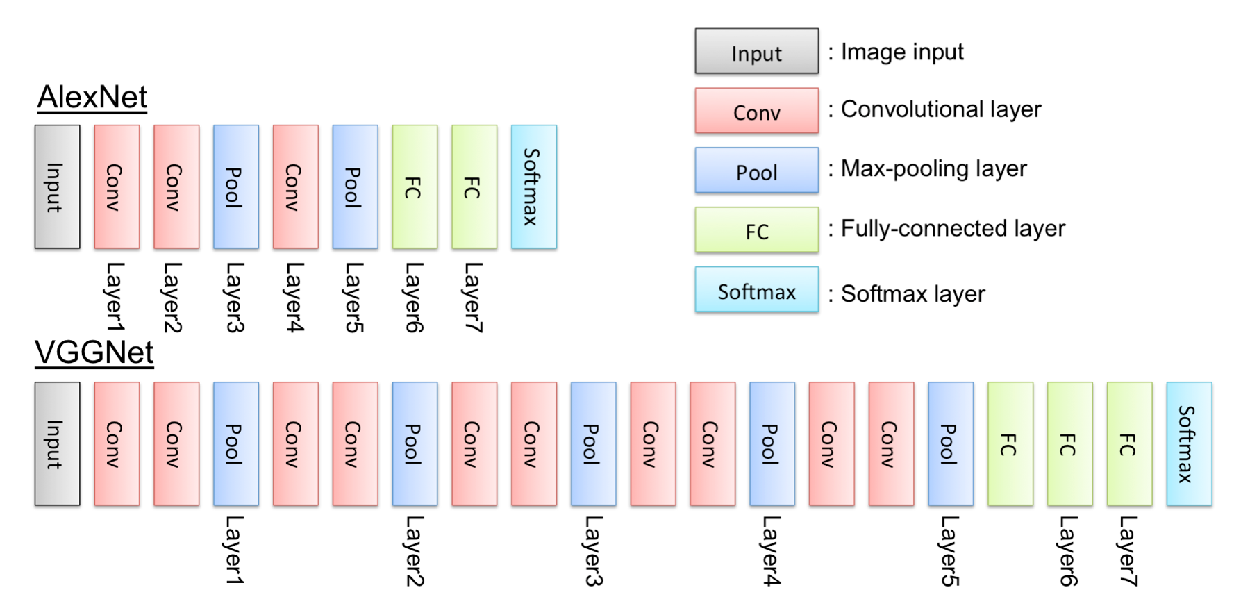
\includegraphics[width=\linewidth]{Images/alex_vgg.eps}
    \caption{Vergelijking van de architectuur van AlexNet en VGGNet}
    \label{fig:alexvgg}
\end{figure}


De representatie die wordt gebruik door Karpathy is de output van VGGNet van de laag voor de softmaxlaag. Dit leidt tot een 4096-dimensionele vector, waarbij elke dimensie kan worden beschouwd als een bepaald concept dat al dan niet aanwezig is in de afbeelding. Deze dimensionaliteit is dezelfde voor alle afbeeldingen, onafhankelijk van de grootte van de input. Dit komt door een herschaling alvorens de afbeeldingsvector te berekenen.

VGGNet is momenteel het best presterende CNN voor afbeeldingsrepresentatie. Wij gebruiken in ons systeem dan ook de afbeeldingsvectoren die berekend zijn met VGGNet. Het berekenen van deze vectoren kan met een implementatie in Caffe.\cite{Jia2014}.

\paragraph{Woordrepresentatie}
Voor het voorstellen van woorden stelt onder andere \todo{de juiste citen} vast dat word embeddings geen toegevoegd waarde brengen. Om die reden gebruikt Karpathy een one-hot encoding waarbij \'e\'en specifieke code behoort tot het start- en stopwoord. Karpathy kiest ervoor om enkel woorden die meer dan vijf keer voorkomen te gebruiken in zijn model. Dit omdat met minder dan vijf woorden, het systeem te weinig voorbeelden heeft om de betekenis en het gebruik van dit woord te leren. Vooraleer een woord als input dient voor het neurale netwerk, vindt eerst nog een vermenigvuldiging plaats met een gewichtsmatrix en een sommatie met een biasvector. Deze gewichtsmatrix en vector trainen mee tijdens de terugpropagatie van het netwerk. Op deze manier is het mogelijk dat semantische verbanden tussen de woordrepresentaties, net als bij word embeddings, toch aanwezig zijn.

\paragraph{Van afbeelding naar beschrijving}
De berekende vector representatie van de afbeelding dient als input voor een recurrent neuraal netwerk. Tijdens de training voorspelt het netwerk het eerste woord op basis van de afbeeldingsvector en een speciale vector die de start van een zin voorstelt. Op basis hiervan voorspelt het model dan wat het volgende woord is. Dit proces herhaalt zich tot het einde van de zin bereikt is. Terugpropagatie op basis van stochastic gradient descent zorgt voor de juiste wijzigingen aan de gewichten van het netwerk. Een eenvoudige weergave van hoe het RNN een beschrijving genereert is te zien op figuur \ref{fig:rnntraining}.

\begin{figure}[tb]
    \centering
    \includegraphics[width=0.5\linewidth]{Images/karpathy.PNG}
    \caption{Generatie van caption met recurrent neuraal netwerk}
\label{fig:rnntraining}
\end{figure}

Het trainen van het RNN gebeurt op basis van de Flickr30k dataset. 
Op basis van een willekeurig gekozen afbeelding uit de trainingsset berekent het netwerk de beste zin. Het verschil tussen deze voorspelling en de correcte zin propageert terug door het netwerk en leidt tot de juiste aanpassing van de gewichten

Wanneer de trainingsset volledig is doorlopen vindt een evaluatie plaats. De perplexity berekend op de resultaten voor de validatieset geeft snel aan of het netwerk nog bijleert of niet. Het systeem slaagt de tussentijdse resultaten op onder de vorm van checkpoints. Deze checkpoints bevatten alle nodige parameters om het opgeslagen model te evalueren. Er is ook de mogelijkheid om de training van het netwerk verder te zetten vanaf een bepaald checkpoint. \todo[inline]{Bij experimenten beschrijven hoe we de beste kiezen}

De code van Karpathy voorziet ook de optie om gebruik te maken van ReLu encoders, deze werken volgens formule $ReLu(x) = max(x,0)$. Er is ook de optie om te kiezen hoe groot de verborgen laag van het RNN moet zijn, alsook de optie om de afbeeldingsrepresentatie al dan niet elke stap toe te voegen.

Formeel gezien berekent het netwerk op basis van input vectoren (woorden in de zin) $(x_1,x_2,...,x_T)$ een reeks van verborgen vectoren $(h_1,h_2,...,h_t)$. Deze verborgen vectoren dienen daarna als de basis voor output $(y_1,y_2,...,y_t)$. Deze outputs worden verkregen door formule \eqref{eq:rnn} te itereren voor $t = 1$ tot $T$.

\begin{equation}
\begin{aligned}
     b_v &= W_{hi} [CNN_{\theta_c}(I)] \\
     h_t &= f(W_{hx} x_{t} + W_{hh} h_{t-1} + b_h + \mathbbm{1}{(t=1)} \odot b_v) \\
     y_t &= softmax( W_{oh} h_t + b_o)
\end{aligned}
\label{eq:rnn}
\end{equation}

In deze vergelijkingen zijn $W_{hi}, W_{hx}, W_{hh}, W_{oh}$ en $b_h, b_o$ parameters die het netwerk leert. De $W_{xy}$ zijn gewichtsmatrices, terwijl $b_i$ bias vectoren zijn. $CNN_{\theta_c}(I)$ is de output van de laatste laag van VGGNet en $f$ is een activatiefunctie. De output komt overeen met een kansverdeling over de verschillende woorden uit de dataset. Er is ook \'e\'en extra dimensie toegevoegd voor het END symbool dat het einde van een zin aangeeft. 

Karpathy schrijft in zijn paper dat het eenmalig gebruiken van de afbeeldingsvector het beste resultaat geeft. Om dit te verifi\"eren hebben wij beide situaties vergeleken. Bij het gebruik van de afbeelding in elke stap verandert het tweede deel van formule \eqref{eq:rnn} in formule \eqref{eq:rnnfeedalways}.

\begin{equation}
     h_t = f(W_{hx} x_{t} + W_{hh} h_{t-1} + b_h + b_v)
\label{eq:rnnfeedalways}
\end{equation}

\todo{Dit is niet echt hoe het werkt}
\todo{nu wel denk ik? }
Het genereren van beschrijvingen gebeurt op basis van beam search. Hierbij bepaalt de output van het netwerk de meest waarschijnlijke eerste woorden voor de zin. De beste $n$ woorden uit die ranking dienen dan als startpunt van de volgende iteratie. Op basis van deze woorden genereert het systeem alle mogelijke opeenvolgingen van twee woorden en voegt deze toe aan de lijst met zinnen bestaande uit \'e\'en woord. Het algoritme gaat door met de $n$ meest waarschijnlijke combinaties, die dus kunnen bestaan uit \'e\'en of twee woorden. Dit proces herhaalt zicht tot alle zinnen een END symbool voorspellen en dus volledig zijn, of tot een maximaal aantal iteraties bereikt is. 
 

\subsection{Long Short Term Memory Netwerk}
\label{sec:lstm}
De code van Karpathy werkt ook met een tweede type van neuraal netwerk dat we gebruikt hebben als startpunt voor onze extensies. Dit netwerk volgt de methode van Vinyals et al.\cite{Google} Het betreft een implementatie van een Long Short Term Memory neuraal netwerk. 

De gebruikte afbeeldingsrepresentatie is dezelfde als bij de RNN implementatie. We gebruiken de 4096-dimensionale feature vectors berekend met VGGNet. 

\paragraph{Van afbeelding naar beschrijving}
Anders dan het RNN van Karpathy, wordt de afbeeldingsrepresentatie beschouwd als het eerste woord in de zin. Daarnaast gebruikt het een LSTM als taalmodel, een uitbreiding van een RNN. Op elk moment bevat het netwerk kennis over alle observaties tot op het huidige tijdstip. Door middel van \emph{gates} is er controle over het al dan niet onthouden van bepaalde waarden. De gebruikte formules, samen met theoretische verduidelijking van het concept, zijn te vinden in sectie \ref{sub:lstm}.

De training van het netwerk verloopt net als bij de RNN implementatie. Het netwerk leert op basis van de Flickr30k training set en bij elke volledige doorloop van de trainingset berekenent de software de perplexity van de resultaten op de validatieset. Dit kan dienen als een criterium om de training stop te zetten. Voor een betere criterium om de training te stoppen verwijzen we u door naar hoofdstuk \ref{cha:experimenten} dat de experimenten in detail beschrijft. %Verder in deze thesis beschrijven we een betere manier om te bepalen wanneer de training moet stoppen.\todo{laatste zin zou k anders doen}

\todo[inline]{de volgende zin heb k hier gezet, maar het hoort ni echt ergens bij :P }
Karpathy voorziet in zijn code ook de mogelijkheid om de hyperbolische tangens te berekenen van de geheugenwaarde van de cel alvorens de output te berekenen. \todo[inline]{Is dit ni gewoon een andere activatiefunctie?} \todo[inline]{mss gewoon weglaten.}

Het genereren van nieuwe beschrijvingen voor ongeziene foto's gebeurt op exact dezelfde manier als bij RNN. Beam search bepaalt de meest waarschijnlijke zin op basis van de uitkomst van het netwerk.



\section{Latent Dirichlet Analysis}
Het gebruik van Latent Dirichlet Analysis op een set van afbeeldingen en beschrijvingen heeft een groot voordeel in de taak van het genereren van nieuwe beschrijvingen. De topicverdelingen bevatten extra semantische informatie die zeer bruikbaar kunnen zijn voor het genereren van beschrijvingen.

 Deze sectie beschrijft hoe LDA zorgt voor extra semantische informatie.

\subsubsection{Berekening van topicverdeling}
\label{subs:Berekening van topicverdeling}
Het leren van het gebruikte LDA model gebeurt op de Flickr30k dataset. Een voorbereidingsproces bewerkt de data zodat deze klaar is voor LDA. Dit proces combineert de vijf captions tot \'e\'en zin, verwijdert stopwoorden stemt de woorden met behulp van een Porter stemmer. \todo{reference naar porter stemmer ?} Deze zinnen vormen de documenten voor het LDA algoritme. Het doel is om op basis van een document te kunnen bepalen welke topics het sterkst aanwezig zijn. Het idee hierachter is dat een topicverdeling ervoor kan zorgen dat het systeem woorden genereert die binnen het juiste topic passen.

Vervolgens begint het trainingsproces. Het aantal topics waarmee het systeem getraind wordt is variabel, en een schatting van het optimale aantal wordt gemaakt op basis van manuele evaluatie, zoals beschreven in sectie \ref{subs:Evaluatie}. Op basis van de zinnen uit de trainingsset berekent het algoritme de topic-woord verdelingen en de sentence-topic verdelingen. Deze verdelingen, berekend op de trainingsset, leiden tot de berekening van de topic-verdelingen voor de test- en validatieset. De ``ground truth'' waarden van de sentence-topic verdelingen voor test- en validatieset worden berekend en opgeslagen.

Bij input van een nieuwe, ongeziene afbeelding moet het systeem in staat zijn om een topicverdeling af te leiden. Daarom is er een link nodig tussen een afbeeldingsrepresentatie en een topicverdeling. Hiervoor gebruiken we een simpel feed-forward neuraal netwerk. Op basis van de eerder berekende ``ground truth'' waarden voor de validatieset leert dit netwerk een mapping van afbeeldingsvector naar topicverdeling. Door middel van terugpropagatie worden de gewichten aangepast. Een vergelijking van negatieve logwaarschijnlijkheid leidt tot een optimalisatie van het aantal hidden layers en van de trainingssnelheid van het netwerk. Dit netwerk kan dan op het moment van testen zeer snel een topicverdeling bepalen voor een ongeziene afbeelding.

Het uiteindelijke netwerk bestaat uit een inputlaag, een verborgen laag met 256 knopen en een outputlaag. De verborgen laag gebruikt de sigmo\"idefunctie \eqref{eq:sigmoid} als transferfunctie, terwijl de outputlaag een softmaxfunctie gebruikt, zoals uitgelegd in sectie \ref{par:softmax}.

\begin{equation}
    \sigma(t) = \frac{1}{1 + e^{-t}}
    \label{eq:sigmoid}
\end{equation}

\subsubsection{Evaluatie}
\label{subs:Evaluatie}
\todo[inline]{herschrijven :(}
De correctheid van de berekende topicverdelingen is uiteraard een kritiek punt in de performantie van het systeem. Daarom hebben we manueel twee testen uitgevoerd. Een eerste test gaat over de optimalisatie van het aantal gebruikte topics. Bij de tweede test controleren we of de topicverdelingen die voorspeld worden door het perceptron wel passen bij de gegeven afbeelding.

Het optimaliseren van het aantal topics gebeurt op basis van manuele analyse van de woorden die voorkomen in elk topic. Op basis van de tien meest voorkomende woorden per topic proberen we een overkoepelend concept te benoemen. Hoe kleiner het aantal topics, hoe moeilijker het is om een sluitende omschrijving van elk topic te vinden. Concreet hebben we getest met 50, 80 en 120 topics. Bij 50 topics is er een terugkerend probleem: topics lijken samengevoegd te zijn. Heel concreet zijn er volgende topics (enkel de 10 meest voorkomende woorden zijn weergegeven): \\
\texttt{jump air leap high midair bubble blow fly wed bride}
\\
waarbij er duidelijk referenties zijn naar springen, bellen blazen en trouwen. Een ander treffend voorbeeld is \\
\texttt{talk man drink cellphone phone hold glass bottle bar beer}
\\ dat duidelijk refereert naar praten en drinken.

Bij het gebruik van 80 topics is dit fenomeen amper aanwezig, en bij het gebruik van 120 topics zijn er meerdere topics waar de top 10 uit ongeveer dezelfde woorden bestaat. Aangezien enkel de top 10 woorden werden geanalyseerd is het waarschijnlijk dat er tussen de verschillende gelijkaardige topics kleine nuances te zien zijn. Op basis hiervan hebben we besloten om het systeem te trainen met verdelingen met 80 en 120 topics. Meer dan 120 trekt naar onze mening de topics te hard uit elkaar, waardoor ook de kansverdeling over de verschillende topics harder wordt afgevlakt. Er zou zich dan een probleem kunnen vormen tijdens het genereren dat bepaalde woorden niet worden gebruikt omdat de topics net niet goed genoeg zijn terwijl de woorden wel perfect kunnen beschrijven wat er op de foto staat.

\section{Flickr30k Entities}
De dataset \emph{Flickr30k Entities}\cite{Plummer2015} is gebaseerd op de Flickr30k dataset. Ze bevat een groot aantal annotaties en bounding boxes, alsook links tussen beide. In deze sectie beschrijven we deze dataset in meer detail. Vervolgens volgt een bespreking van de pogingen om deze grote hoeveelheid informatie te verwerken naar een handelbaar formaat.

\subsection{Dataset}
\label{sub:Dataset}
Flickr30k Entities is ontstaan op basis van een eenvoudig idee. De makers zien in dat een ``standaard'' afbeeldingsbeschrijvend systeem een globaal verband leert tussen een foto en een zin, zonder echt rekening te houden met de overeenkomsten tussen entiteiten op de foto en in de zin. Er zijn vrij recent wel een aantal systemen ontwikkeld die een mapping maken van afbeeldingsregio's naar beschrijvingen. Deze systemen veronderstellen echter dat deze verbanden latent zijn. Hier probeert de nieuwe Entities dataset verandering in te brengen, door de verbanden tussen beschrijving en foto te expliciteren.

De dataset is gebaseerd op de meer dan 30,000 afbeeldingen uit de Flickr30k\cite{Young2014} dataset met de bijhorende beschrijvingen. De makers brengen een uitbreiding hiervan, met een set van bijna 250,000 coreference chains, die verbanden aangeven tussen regio's uit de afbeeldingen en zinsdelen uit de beschrijvingen. Deze aanpak lijkt op wat de MS COCO\cite{Lin2014} dataset biedt, maar de objecten in de COCO dataset zijn onafhankelijk van de beschrijvingen gedetecteerd. Figuur \ref{fig:entities} toont een aantal voorbeelden van annotaties en references uit de Entities dataset, terwijl figuur \ref{fig:cocoexamples} toont hoe de verschillende objecten in de COCO dataset worden opgeslagen. Het is duidelijk dat er bij de COCO dataset geen rechtstreeks verband is met de beschrijvingen. 

\begin{figure}[!tb]
    \centering
    \begin{tabular}[t]{cc}
      \includegraphics[height=3.0in]{Images/example_hat.png} \vspace{-3mm}&
      \includegraphics[height=3.0in]{Images/example_parade.png}\\
      \includegraphics[valign = T,width=.4\columnwidth]{Images/example_hat_text.pdf}&
      \includegraphics[valign = T,width=.4\columnwidth]{Images/example_parade_text.pdf}
  \end{tabular}
\caption{Voorbeelden van Flickr30k Entities annotaties. De kleur van de frases is overeenkomstig de kleur van de bounding boxes op de afbeelding.\cite{Plummer2015}}
\label{fig:entities}
\end{figure}

\begin{figure}
    \centering
    \subfloat{
        \includegraphics[width=0.47\linewidth]{Images/coco_example1.png}}\hfill
    \subfloat{
        \includegraphics[width=0.47\linewidth]{Images/coco_example2.png}}
    \caption{Voorbeelden van geannoteerde afbeeldingen uit MS COCO dataset. Elk gekleurd object behoort tot \'e\'en van de objectcategorie\"en gedefinieerd door de makers.}
    \label{fig:cocoexamples}
\end{figure}



\subsection{Gebruik}
\label{sub:Gebruik}
\todo{probeer hier is nen hele hoop 'we's uit te halen...}
Deze dataset bevat zeer veel extra informatie verspreid over een grote hoeveelheid references. Een probleem dat zich voordoet is dat sommige van de bounding boxes zo klein zijn dat er amper informatie uit te halen is. Daarom is er een reductie uitgevoerd van de dataset alvorens over te gaan tot het verwerken van de data. 

Deze reductie gebeurt op basis van de grootte van de bounding box. Een deel van de bounding boxes zijn slechts enkele pixels hoog of breed, waardoor een CNN hier weinig informatie kan uithalen. Deze bounding boxes worden dus uit de dataset verwijderd. De limiet van zichtbaarheid en informatief zijn van een afbeelding staat ter discussie, maar wij kozen om alles kleiner dan 64 bij 64 pixels te verwijderen, wat resulteerde in 190,000 te gebruiken bounding boxes en corresponderende frases. 

De dataset is beschikbaar als tekstbestanden die weergeven welke bounding boxes op welke afbeelding te zien zijn, en met welke delen van de beschrijving elke box overeenkomt. Er zijn een aantal boxes die wel zijn opgenomen in de dataset, maar geen overeenkomstig zinsdeel hebben. De semantische meerwaarde van dergelijke boxes is miniem, dus horen deze ook niet tot de bekeken verzameling. 

Om de data bruikbaar te maken voor verwerking leest een script de tekstbestanden uit, en slaat alle bounding boxes op als aparte afbeelding. Op basis van die afbeeldingen berekent de Caffe-implementatie van VGGNet een vectorrepresentatie. De overeenkomstige zinsdelen zijn omgezet naar een tf-idf gewogen vectorweergave. 

Op basis van de CCA-uitbreiding beschreven in sectie \ref{sub:stackedcca} berekenen we een geaugmenteerde representatie van de afbeeldingen uit de Flickr30k dataset. De extra informatie uit de overeenkomsten tussen bounding boxes en frasen zit vervat in een eerste gemeenschappelijke CCA ruimte. Op basis van \cite{Gong2014} berekenen we een representatie van de trainingsafbeeldingen, waarin ook de informatie uit de Entities dataset aanwezig is.

Het berekenen van de CCA mapping tussen de bounding boxes en de frasen uit de Entities dataset verliep zonder problemen. De berekening van de augmentatie was ook probleemloos, maar tijdens het berekenen van de CCA mapping tussen de augmentaties van de Flickr30k foto's en hun beschrijvingen zijn we tot de conclusie gekomen dat het, door de hoge dimensionaliteit, qua tijdsbestek onhaalbaar was om deze mapping te gebruiken in onze experimenten. 



\section{Canonical Correlation Analysis}
Het toevoegen van extra semantische informatie kan gebeuren op verschillende manieren. Een eerste optie is LDA, zoals eerder beschreven. Er kan echter ook gebruik gemaakt worden van CCA. Waar LDA focust op het blootleggen van verbanden tussen de woorden uit de captions, berekent CCA een ruimte die tussen de afbeelding en de zin ligt.

Het berekenen van deze tussenliggende ruimte gebeurt in twee stappen. Het eerder vernoemde VGGNet berekent de afbeeldingsvectoren voor de traininggset. Een door tf-idf gewogen vector stelt de bijhorende zinnen voor, zoals eerder beschreven. Deze voorstelling is gebaseerd op twee belangrijke principes. Ten eerste is het gewicht van een woord in een zin proportioneel met het aantal keer dat het woord voorkomt in het document (term frequentie of tf). Ten tweede is het gewicht invers gerelateerd aan het aantal documenten waar het in voorkomt (inverse doucment frequentie of idf). Een woord dat in alle documenten voorkomt dient een lager gewicht te krijgen dan een woord dat slechts in een fractie van de documenten voorkomt.

Belangrijk is dat alle zinnen apart worden beschouwd. Waar bij LDA de vijf zinnen per afbeelding worden gereduceerd tot \'e\'en zin, blijven ze hier apart. Dit om ervoor te zorgen dat de mapping rekening houdt met de verschillende zinnen, moest er sprake zijn van heel verschillende formuleringen van dezelfde concepten. Meer concreet houdt dit in dat elke foto maximaal gecorreleerd dient te zijn met vijf verschillende zinnen uit de trainingsset.

Een deel van de rijkdom van de dataset gaat verloren als er gebruikt wordt gemaakt van een aaneensluiting van de verschillende zinnen. Bij LDA doet dit probleem zich niet voor, en is het zelfs beter om de zinnen bij elkaar te voegen, angezien we \'e\'en topicverdeling per afbeelding beogen, en niet per zin. Synoniemen en afgeleiden worden beschouwd als deel van hetzelfde document, juist door de aaneensluiting van de zinnen.

Na het berekenen van de representaties van afbeeldingen en zinnen volgt een berekening van de correlatiecomponenten. Dit gebeurt met de \texttt{MATLAB}-implementatie van het canonical correlation algoritme. Het resultaat bestaat uit twee projectiematrices, die dienen om afbeeldings- en beschrijvingsvectoren te projecteren op de tussenliggende ruimte die de correlatie maximaliseert. Voor onze experimenten maken we enkel gebruik van de projectie voor afbeeldingen, aangezien Jia et al.\cite{Fernando2015} aantonen dat het gebruik van enkel de afbeeldingsprojectie de beste resultaten oplevert.


\section{Toevoeging van LDA topicverdeling aan RNN}
De eerder berekende topicverdelingen kunnen dienen als extra semantische informatie om de generatie in de juiste richting te sturen. Het integreren van de topicverdeling $L$ in het RNN gebeurt volgens formule \eqref{eq:rnnldaonce} die het tweede deel van \eqref{eq:rnn} vervangt. Het rode deel in de formule duidt de verschillen met \eqref{eq:rnn} aan. $W_l$ is een gewichtsmatrix voor vermenigvuldiging met de topicverdeling.

\begin{equation}
    h_t = f(W_{hx} x_{t} + W_{hh} h_{t-1} + b_h + \mathbbm{1}{(t=1)} \odot b_v +\color{red}{\mathbbm{1}{(t=1)} \odot W_lL}
    \color{black}
    \label{eq:rnnldaonce}
\end{equation}

Er kan ook gekozen worden om de topicverdeling elke stap toe te voegen, wat leidt tot formule \eqref{eq:rnnldaall}. Het lijkt ons interessant om te experimenteren met het al dan niet altijd toevoegen van de topic informatie. Dit kan, in tegenstelling tot het steeds toevoegen van de afbeelding, een verbetering betekenen. De informatie uit de topicverdeling is afgeleid van de afbeelding, maar bevat informatie van een lagere dimensionaliteit. Het herhaaldelijk meegeven van de topic vector zorgt dat het netwerk elke stap deze semantische informatie binnenkrijgt. Voor een gedetailleerde beschrijving van de uitgevoerde experimenten, en een vergelijking tussen de verschillende settings verwijzen we u door naar hoofstuk \ref{cha:resultaten}.


\begin{equation}
    h_t = f(W_{hx} x_{t} + W_{hh} h_{t-1} + b_h + \mathbbm{1}{(t=1)} \odot b_v + W_lL
    \label{eq:rnnldaall}
\end{equation}


\section{gLSTM}
\subsection{Guided LSTM}
Guided Long Short Term Memory (gLSTM) is een recente uitbreiding van het LSTM model ge\"introduceerd door Jia et al.\cite{Fernando2015} In dit model extraheren ze eerst semantische informatie van elke afbeelding. Deze informatie dient dan als extra input of ``gids'' voor het LSTM-blok.

Na het bestuderen van bestaande LSTM-modellen ontdekten de auteurs dat de gegenereerde zinnen ``semantische drift'' vertonen. Dit wil zeggen dat naarmate de zin evolueert, de betekenis van volgende woorden steeds minder met de input-afbeelding te maken heeft. Ze vermoeden dat dit komt door twee tegenwerkende krachten. Enerzijds moet de zin de afbeelding beschrijven, anderzijds moet de zin passen in het taalmodel. Om die reden introduceren ze een semantische gids, die ervoor moet zorgen dat het model na enkele woorden op het juiste pad blijft. Dit gebeurt door aan woorden die semantisch verbonden zijn aan de afbeelding een positieve bias te geven.

Ze gebruiken vier verschillende semantische gidsen in hun experimenten. Als eerste model gebruiken ze een ``retrieval-based'' gids. Hierbij zoeken ze eerst naar zinnen die gerelateerd zijn aan de afbeelding. Vervolgens verzamelen ze daaruit de zinnen met de hoogste rang. Deze zinnen vormen dan de extra input.
Als tweede model leren ze eerst een CCA-model. Vervolgens nemen de auteurs de projectie van de afbeeldingsrepresentatie in de gemeenschappelijke ruimte. Daarna worden de dichtstbijzijnde geprojecteerde zinnen gezocht op basis van cosinusgelijkheid. Ook hier vormen de hoogst scorende zinnen de extra input.
Een derde model gebruikt de CCA-projectie van de afbeelding in de gemeenschappelijke ruimte rechtstreeks als gids.
Als laatste model gebruiken ze de afbeeldingsrepresentatie zelf als gids.

Om dit te implementeren starten ze net als in deze masterproef van de LSTM-implementatie van Karpathy. Ze defin\"ieren de geheugencellen en poorten zoals in de volgende formules. Hierbij zijn de rode delen toevoegingen ten opzichte van Vinyals et al.\cite{Google} \todo{misschien referentie naar deze formules in theorie?}:

%
\begin{eqnarray}
\vspace{-3mm}
\label{glstm-memory-start}
i_l' & = & \sigma (W_{ix} x_l + W_{im} m_{l-1} \color{red}{+ W_{iq} g}) \label{glstm-input} \\
f_l' & = & \sigma (W_{fx} x_l + W_{fm} m_{l-1} \color{red}{+ W_{fq} g}) \\
o_l' & = & \sigma (W_{ox} x_l + W_{om} m_{l-1} \color{red}{+ W_{oq} g}) \\
c_l' & = & f_l' \odot c_{l-1}' + i_l' \odot h(W_{cx} x_l + \nonumber \\
&   & + W_{cm} m_{l-1} \color{red}{+ W_{cq} g}) \\
m_l & = & o_l' \odot c_l'
\label{glstm-memory}
\vspace{-3mm}
\end{eqnarray}
\todo{Formules bij LSTM zelf + meer uitleg bij gebruikte dinges}
\todo{gebruikte dinges. zo heerlijk specifiek}
Hierbij is $g$ de vectorvoorstelling van de semantische informatie. De gids is onafhankelijk van de tijdstap en werkt dus globaal voor elke afbeelding. Figuur \ref{fig:glstm} geeft een visuele voorstelling van de gLSTM-blok.

\begin{figure}[tb][h]
	\centering
	\includegraphics[width=\linewidth]{Images/glstm.pdf}
	\caption{LSTM-blok in het zwart. Uitbreidingen van gLSTM in het rood.}
	\label{fig:glstm}
\end{figure}

Jia et al. bekomen zeer goede resultaten. De eerste drie gidsen zorgen voor verbetering op hun baseline. Enkel de afbeelding als gids zorgt voor verslechtering. De rechtstreekse CCA-projectie presteert het beste.

\subsection{gLSTM met LDA en CCA}
Net als Jia implementeren we de gLSTM als een uitbreiding van LSTM overeenstemmend met formules \ref{glstm-memory-start}-\ref{glstm-memory}.
Om te kunnen vergelijken met hun paper kan onze implementatie ook de CCA-projectie als gids gebruiken.
Daarnaast veronderstellen we dat LDA een goede bron van semantische informatie is. Het bevat immers een verdeling van de onderwerpen die aanwezig zijn in de afbeelding. Daarom kan LDA ook als gids worden gekozen.
We maken dus twee modellen zodat het mogelijk is om na te gaan of LDA een betere gids is dan CCA in onze configuratie van de gLSTM.

\section{Normalisatie van beam search}
Naast het introduceren van gLSTM's breiden Jia et al. \cite{Fernando2015} de implementatie van Karpathy nog op een tweede manier uit. Na evaluatie van bestaande modellen leidden ze af dat het gebruikte beam-search algoritme een voorkeur heeft voor kortere zinnen. Beam-search neemt de som van de log-likelihood van individuele woorden als criterium. Aangezien deze waarde voor elk woord negatief is, zal het algoritme sneller kiezen om te stoppen. Om dit fenomeen tegen te gaan introduceren ze de genormaliseerde log-likelihood van elk woord als criterium.
\todo[inline]{hier moet volgens mij meer uitleg bij de formule :(}

\begin{equation}
p = \frac{1}{\Omega(\ell)}\sum_{l=1}^{\ell} \log p(s_l | x, s_{1:l}, \theta)
\label{eq:log-sentence-norm}
\end{equation}

De auteurs van de paper bestuderen meerdere functies voor $\Omega$. Wij implementeren de twee meest performante.
Enerzijds gebruiken we de Gaussiaanse functie $\Omega(\ell) \sim \mathcal{N}(\mu, \sigma)$, waar $\mu$ en $\sigma$ respectievelijk het gemiddelde en de standaardafwijking zijn van de lengtes van de zinnen in het trainingscorpus. Hierdoor moeten gegenereerde zinnen gelijkaardige lengtes hebben aan deze uit het corpus. 
Anderzijds implementeren we de min-hinge normalisatie. Met deze methode is de normalisatiefactor gelijk aan de gemiddelde lengte van het trainingscorpus ($\mu$) als de zin langer is dan dit gemiddelde. Indien de zin korter is, is de factor gelijk aan de lengte van de zin. Dit komt overeen met de functie $\Omega(\ell)=\min\{\ell, \mu\}$.

Een eigen implementatie van de $\Omega(\ell)$ functie is gebaseerd op de hoeveelheid informatie die in elk woord is vervat. Op basis van de trainingsset bepalen we de tf-idf gewichten van elk woord. Op basis van deze gewichten is het mogelijk om een score te berekenen voor de gegenereerde zinnen. Het doel hiervan is om de zinnn zoveel mogelijk informatie te laten bevatten. Hoe hoger de gecombineerde tf-idf score van een zin, hoe meer informatie. 
\todo[inline]{meer}

\section{FSMN}
E\'en van de eerste wijzigingen die we in deze thesis probeerden te implementeren, waren Feedforward Sequential Memory Neural Networks (FSMN)\cite{Zhang}. Deze netwerken vormen een uitbreiding op gewone feed-forward neurale netwerken. Dit netwerk kan afhankelijkheden op lange termijn leren zonder recurrente verbindingen te gebruiken. Het doet dit door sequenti\"ele geheugenblokken in de verborgen lagen van het feed-forward netwerk te steken. 

Volgens de paper zijn deze netwerken in staat om betere en vooral snellere resultaten te leveren dan de huidige RNN-modellen. De snellere resultaten zijn mogelijk omdat gebruik kan worden gemaakt van standaard terugpropagatie zonder dat er zich problemen voordoen door de recurrente verbindingen. Figuur \ref{fig:fsmn} toont de  algemene structuur van dit netwerk. Hierbij dient de output van een verborgen laag als input voor een geheugenblok. Dit geheugenblok is in staat om informatie bij te houden van meerdere vorige inputs. Het geheugenblok dient dan zelfs als extra invoer voor een volgende laag.

Vooral de snellere resultaten leken zeker een goede uitbreiding voor het model van Karpathy. Trainen van een RNN batch duurt immers ongeveer 4 seconden en voor LSTM 7 seconden. Hierdoor duurt het volledig trainen van het neuraal netwerk gemiddeld meer dan zeven dagen.
Hoewel de implementatie van dit netwerk op basis van de paper succesvol was, vertoonden de resultaten zowel qua kwaliteit en snelheid geen verbetering. Om die reden hebben we geen verdere experimenten met FSMN's uitgevoerd.

\begin{figure}[tb]
	\centering
	\includegraphics[width=\linewidth]{Images/FSMN}
	\caption{Algemene structuur van Feedforward Sequentieel Geheugen Neural Netwerken.}
	\label{fig:glstm}
\end{figure}

\chapter{Evaluatie}
\label{hoofdstuk:evaluatie}
Om verschillende systemen te vergelijken, moet er een manier zijn om de gegenereerde zinnen te evalueren. Elke zin moet aan twee belangrijke voorwaarden voldoen. Enerzijds moet de inhoud van de zin overeenkomen met de inhoud van de afbeelding. Anderzijds moet de zin een grammaticaal correcte structuur hebben en voldoende vloeiend zijn.
Dit hoofdstuk behandelt enkele gebruikte methodes om de ontwikkelde systemen te evalueren. Twee van deze methodes vinden hun oorsprong in de computervertaling. Ze zijn ontwikkeld om automatisch de kwaliteit van vertalingen te meten. Het doel van deze evaluatiealgoritmes is om zo goed als mogelijk menselijke evaluatiescores te benaderen. De tweede sectie bekijkt enkele nuttige statistieken over de gegenereerde zinnen die peilen naar bepaalde eigenschappen zoals originaliteit. De laatste sectie behandelt een evaluatiemethode die de laatste jaren in onbruik is geraakt binnen dit onderzoeksdomein. Deze vorm van evaluatie kijkt naar het ophalen van afbeeldingen op basis van zinnen en omgekeerd. Hieruit volgt steeds een rangschikking, die leidt tot een numerieke score.


\section{Automatische evaluatie}
Ideaal gezien beoordelen meerdere mensen elke zin om tot een betrouwbare evaluatie van de zinskwaliteit te komen. Deze beoordeling kan bijvoorbeeld door een score te geven op de kwaliteit van elke zin. Een andere optie is om proefpersonen te laten oordelen of een automatisch gegenereerde zin beter, gelijkaardig of slechter is dan de overeenkomstige referentiezin. Het nadeel van elk van deze methodes is de nood aan meerdere proefpersonen die voor elke gebruikte methode of instelling van het model, alle duizend zinnen van de validatieverzameling of de testverzameling moet beoordelen. Het is duidelijk dat dit een kostelijke operatie is. Daarvoor bieden automatische evaluatiealgoritmes een oplossing. Het nadeel van deze methodes is dat ze niet perfect overeenkomen met de menselijke evaluatie.

De rest van deze sectie bevat een bespreking van twee algoritmes uit de computervertaling BLEU\cite{Papineni2001} en Meteor\cite{Denkowski2007a}. Deze algoritmes zijn bruikbaar omdat ze de gegenereerde zinnen beschouwen als ``vertalingen'' van de afbeeldingen. Het is aangetoond dat de twee methodes in zekere mate correleren met menselijke evaluaties van de gegenereerde zinnen. Van de gebruikte methodes heeft Meteor de hoogste correlatie\cite{Elliott2014}.

\subsection{BLEU}
Kort gesteld berekent het BLEU-algoritme scores van computervertalingen op basis van overeenkomsten met de referentiezinnen. Deze overeenkomsten bestaan uit gemeenschappelijke woorden of opeenvolgingen van gemeenschappelijke woorden. Verschillende vormen van BLEU kunnen worden gebruikt afhankelijk van het aantal gebruikte woorden in een opeenvolging. Een opeenvolging van $n$ woorden krijgt de naam \emph{n-gram}. Het redelijk eenvoudige algoritme van BLEU heeft echter wel enkele nadelen.

\subsubsection{Algoritme}
Om de n-gram BLEU-score van een zin te berekenen bepaalt het algoritme eerst de \textit{modified n-gram precision} of gewijzigde n-gram-precisie. Hierbij volgt de precisie uit gemeenschappelijke n-grams. N-gram-precisie houdt bovendien rekening met het aantal keer dat elk woord in de referentiezinnen voorkomt. Op deze manier krijgen zinnen als \texttt{the the the the the} een lage score omdat \texttt{the} nooit vijfmaal voorkomt in een referentiezin. 

De berekening van de gewijzigde n-gram-precisie neemt eerst het maximum van het aantal keer dat een specifieke n-gram voorkomt in elke referentiezin. Vervolgens telt het algoritme het aantal voorkomens ($Count(ngram)$) van deze sequentie in de gegenereerde zin $s$. Het minimum van deze twee getallen ($Count_ {clip}$) wordt dan voor elk woord in de vertaalde zin opgeteld en gedeeld door de som van het totaal aantal n-grams in de gegenereerde zin. Deze score is afhankelijk van de waarde van $n$.

\begin{equation}
p_{modified}(s) =
\frac{\sum\limits_{ngram \in s} Count_{clip}(ngram)}{\sum\limits_{ngram' \in s} Count(ngram')}
\label{formule:ngramprecision}
\end{equation}
Vanuit deze formule volgt een score voor een volledige corpus van gegenereerde zinnen als volgt:
\begin{equation}
p_{n} =
\frac{\sum\limits_{C \in \{Candidates\} } \sum\limits_{ngram \in C} Count_{clip}(ngram)}{\sum\limits_{C' \in \{Candidates\} } \sum\limits_{ngram' \in C'} Count(ngram')}
\label{formule:corpus_modified}
\end{equation}
Hierin is $Candidates$ de verzameling van alle gegenereerde zinnen.

Vanuit deze scores voor $n=1$ tot en met $N$ is het mogelijk om een N-gram BLEU-score te bepalen. Dit gebeurt door het gemiddelde logaritme te nemen met uniforme gewichten $w_n$, wat overeenkomt met het geometrisch gemiddelde van de gewijzigde n-gram-precisies.
\begin{equation}
BLEU = exp(\sum\limits_{n=1}^N w_nlog(p_n))
\end{equation}
Deze score dwingt echter niet de juiste lengte van de zin af. Om die reden bepaalt Papineni een extra multiplicatieve factor, namelijk de \texttt{Brevity Penalty} ($BP$). Voor elke gegenereerde zin bepaalt het algoritme de referentiezin met de dichtstbijzijnde lengte. De lengte daarvan noemt de paper de ``beste match lengte''. Vervolgens telt hij zowel de lengtes van de gegenereerde zinnen als de beste match lengte op tot respectievelijk $c$ en $r$. De onderstaande formule berekent de Brevity Penalty.
\begin{equation}BP=
 \begin{cases}
1 & if c > r \\
e^{1-r/c} & else
\end{cases}
\end{equation}

De uiteindelijke BLEU-N score is dan gelijk aan:
\begin{equation}
BLEU = BP\cdot exp(\sum\limits_{n=1}^N w_nlog(p_n))
\end{equation}
Hierbij is $w_n$ gelijk aan $1/N$ wanneer het uniforme geometrisch gemiddelde wordt genomen.

\subsubsection{Nadelen en gebruik}
De BLEU-score is de meest gebruikte gebruikte evaluatiemethode in de literatuur. De meeste papers die afbeeldingsbeschrijvingen genereren, bespreken BLEU-1 tot BLEU-4 scores. De literatuur lijkt het echter niet eens over het gebruik van de Brevity Penalty. Sommige papers vermelden expliciet dat ze het niet gebruiken, maar andere volgen de paper van Papinemi volledig. Door dit verschil in evaluatie is de vergelijking van verschillende systemen niet altijd eerlijk. Wanneer de gegenereerde zinnen lang genoeg zijn komen de scores wel overeen.
In onze experimenten stellen we de Brevity Penalty steeds gelijk aan 1.

Naast deze problemen bestaan er verschillende implementaties met kleine onderlinge verschillen. De meeste van deze verschillen vinden in hun oorsprong in het al dan niet toevoegen van normalisatie. Hierdoor zijn de concrete scores dus afhankelijk van de gebruikte implementatie. In onze experimenten gebruiken we de \texttt{multi-BLEU.pl}\footnote{\url{https://github.com/moses-smt/mosesdecoder/blob/master/scripts/generic/multi-bleu.perl}} code uit de Moses decoder\cite{Koehn2006}, omdat Karpathy deze ook voorziet in zijn code.

Elliot et al.\cite{Elliott2014} tonen aan dat BLEU-3 en BLEU-4 slechts een matige correlatie heeft met menselijke beoordeling. De correlatie van BLEU-1 en BLEU-2 is nog minder.
Hiervoor zijn meerdere verklaringen mogelijk. Zo kijkt BLEU enkel naar exacte woordovereenkomsten, maar houdt het geen rekening met semantisch gelijkaardige woorden. Het gebruik van een synoniem in plaats van een overeenkomstig woord bijvoorbeeld geeft geen hogere score, terwijl dit bij menselijke evaluaties wel zo is. Daarnaast krijgen woorden die weinig semantische waarde bevatten een evengrote score als woorden die veel meer informatie over de afbeelding geven. Concreet geeft dus een woord als \texttt{a} evenveel extra score als een woord als \texttt{ski}. Ook werkwoorden die semantische informatie bevatten die in de referentiezin als substantief voorkomen geven problemen. Hieronder volgen voorbeelden van situaties waarbij zinnen slecht scoren volgens BLEU, maar inhoudelijk toch hetzelfde weergeven.
\\

Referentie 1: \texttt{Two boys are on their bikes.}

Kandidaat 1: \texttt{Two boys are on their bicycles.}

Referentie 2: \texttt{A man is skiing down a hill.}

Kandidaat 2: \texttt{A man is going down a hill on his skis}
\\

Meteor is een evaluatiealgoritme met als doel het vermijden van dergelijke foute evaluaties.

\subsection{Meteor}
Elliott et al.\cite{Elliott2014} tonen aan dat zeker unigram BLEU (BLEU-1) slechts een zwakke correlatie heeft met menselijke evaluatie. Hogere orde BLEU-scores hebben slechts een matige correlatie. Meteor is een metriek die specifiek ontworpen is om de tekortkomingen van BLEU te verbeteren. Meteor correleert het beste met menselijke evaluatie van de door Elliott onderzochte evaluatiemechanismen.

\subsubsection{Algoritme}
Meteor\cite{Denkowski2007a} evalueert vertaalde zinnen door ze te aligneren met de referenties en van deze alignering per zin een score te berekenen. Bij het berekenen van de score wordt net zoals bij BLEU gekeken naar de precisie. Daarnaast heeft in contrast met BLEU ook de recall een invloed.\todo{wat met recall?} De paper bevat een implementatie in de vorm van een JAR-bestand, zodat er geen twijfel bestaat over het gebruik van het algoritme.

Concreet probeert het algoritme twee zinnen te aligneren met behulp van vier ``matchers''. Als eerste is er een match wanneer twee woordvormen exact dezelfde zijn. Als tweede is er een match wanneer met een Snowball Stemmer\cite{porter2001snowball} ``gestemde'' woorden gelijk zijn. Een derde matcher kijkt naar overeenkomsten in de WordNet synoniemenlijst van elk woord\cite{Miller1990}. Als laatste vormen frases of woordsequenties een match wanneer ze in zogenoemde parafrasetabellen voorkomen. Een parafrasetabel bevat paren van frases en overeenkomstige parafrases. Parafrases zijn woordsequenties die dezelfde betekenis hebben dan de overeenkomstige frase, maar anders geformuleerd zijn.
Elke matcher heeft een bepaald gewicht. De experimenten gebruiken de standaardgewichten van Meteor 0.85, 0.2 ,0.6 en 0.75.

Uiteindelijk worden alle matches gegeneraliseerd tot frase matches met een bepaalde startpositie en eindlengte. Een van de doelen van de Meteor score is om zoveel mogelijk woorden af te dekken in de twee zinnen. Daarnaast moet het aantal \textit{chunks} minimaal zijn. Denkowski et al. defini\"eren een chunk als aaneengesloten en identiek geordende matches tussen de twee zinnen. De uiteindelijke Meteor score bestaat uit de F-score $F_{mean}$ vermenigvuldigd met een penalisatiefactor $Pen$ op basis van het aantal chunks.


\begin{equation}
Score = (1 - Pen)*F_{mean}
\end{equation} 
\begin{equation}
Pen = \gamma (\frac{ch}{m})^\beta 
\end{equation}
\begin{equation}
F_{mean} = \frac{PR}{\alpha P + (1- \alpha)R}
\end{equation}
Hierbij zijn $P$ en $R$ respectievelijk de gewogen precisie en recall van de gealigneerde unigrams ($m$) tussen kandidaat- en referentiezin. $m$ is het gemiddeld aantal gematchte woorden. $ch$ is het aantal chunks. $\alpha$,$\beta$ en $\gamma$ zijn vooraf getrainde parameters.

Wanneer er meerdere referenties zijn in het corpus, bepaalt het maximum van de individuele scores van elke referentie de score van de vertaling.

\subsubsection{Gebruik en nadelen}
Zoals al aangehaald toonden Elliott en Keller in 2014 aan dat van de bestudeerde evaluatiemethodes Meteor de hoogste correlatie heeft met menselijke beoordelingen voor afbeeldingsbeschrijvingen. Om deze reden rapporteren wij ook de resultaten met dit algoritme. In de literatuur blijven BLEU-scores echter de meest gerapporteerde resultaten.

Ondanks dat het het meest performante algoritme is, vertoont Meteor nog steeds slechts matige correlatie met menselijke beoordelingen. Verder onderzoek naar betere automatische evaluatie kan dus nuttig zijn. Daarnaast vereist het tabellen en synoniemenlijsten die niet voor elke taal beschikbaar zijn. Voor het Engels is deze informatie wel beschikbaar. 


\section{Extra informatie uit de gegenereerde zinnen}
Naast de automatische algoritmes die aan elk model een duidelijke score geven, bevatten de gegenereerde zinnen nog andere interessante statistieken. Deze statistieken hebben niet altijd een rechtstreeks verband met de kwaliteit van de zinnen. Ze geven wel informatie die nuttig kan zijn om het gebruikte model te analyseren en te verbeteren.

Een eerste vorm van informatie ligt in de verdeling van de lengtes van de zinnen. Ons systeem biedt de mogelijkheid om voor elke aanwezige lengte in de bestudeerde verzameling het aantal zinnen te bepalen. Hierdoor is het onder andere mogelijk om uitschieters vast te stellen. Ook maakt het de detectie van vermoedelijk foutieve zinsconstructies mogelijk. Het aantal zinnen van lengte twee, drie of bijvoorbeeld meer dan twintig geeft een goede indicatie van de neiging om inhoudsloze zinnen te genereren. Daarnaast berekent het systeem ook de gemiddelde lengte en vergelijkt het deze met de gemiddelde lengte van de referentiezinnen. Dit maakt duidelijk of het model een voorkeur heeft voor bijvoorbeeld korte zinnen.

De gebruikte woordenschat en bijbehorende woordfrequenties bieden een tweede bron van informatie. Het aantal unieke woorden geeft een idee van hoe gevarieerd het woordgebruik is van het model. Als dit aantal aan de lage kant is, is de kans groter dat het model veel dezelfde uitdrukkingen en bij uitbreiding zinnen genereert. Daarnaast zal het niet in staat zijn om uitzonderlijke foto's correct te beschrijven. Het aantal voorkomens van de gebruikte woorden geeft informatie over de voorkeur voor bepaalde woorden. De vergelijking van deze voorkeur met deze van de referentiezinnen leidt tot de ontdekking van bepaalde eigenschappen van het model.

Een derde optie kijkt hoeveel unieke zinnen het systeem genereert. De implementatie biedt de mogelijkheid om de gegenereerde zinnen voor de testverzameling te vergelijken met die in de trainingsverzameling. Dit geeft een beeld van de mate waarin het model nieuwe zinnen genereert of gekende zinnen teruggeeft. Daarnaast is er de mogelijkheid om het aantal volledig unieke zinnen te berekenen. Dit zijn zinnen die niet in de trainingsverzameling voorkomen of al gegenereerd zijn. Zo is het mogelijk om een beeld te vormen van hoe creatief het systeem is in het genereren van zinnen. 

\section{Afbeelding-zin rangschikking}
Enkele oudere werken in de literatuur over automatische afbeeldingsbeschrijving gebruiken nog een andere vorm van evaluatie. Hodosh introduceerde deze vorm van evolueren voor dit type van problemen\cite{Hodosh2013}. Hij defini\"eert twee types van evaluatie op basis van het opzoeken van een gezochte zin of afbeelding. Enerzijds met als startpunt een afbeelding, waarbij beschrijvende zinnen worden gezocht (sentence retrieval). Anderzijds zoekt hij afbeeldingen op basis van een zin (image retrieval). Voor afbeeldingen moet een systeem een rangschikking van de zinnen bij elke foto produceren. Vervolgens vormt de positie $r$ van de eerste correcte zin de basis van de score. De eenvoudige maar veelgebruikte metriek $recall @ k$ wordt gebruikt voor evaluatie. Hierbij vormt het percentage van de afbeeldingen waarbij de correcte zin bij de eerste $k$ zinnen zit de uiteindelijke score. Ook de mediaan van de gevonden posities ($med\: r$)wordt dikwijls vermeld. Hetzelfde principe werkt ook in de omgekeerde richting. Hierbij gaat het model op basis van een zin naar een rangschikking van de afbeeldingen. Deze laatste manier van evalueren toont aan hoe het gebruikte model kan worden gebruikt om afbeeldingen te zoeken op basis van nieuwe queries. 

Volgens Vinyals et al.\cite{Google} is de transformatie van generatie naar rangschikking echter geen gerechtvaardigde evaluatiemethode. Naarmate afbeeldingen en daarbij ook het woordenboek complexer worden, groeit het aantal mogelijke zinnen exponentieel. Hierdoor daalt de waarschijnlijkheid van de voorgedefin\"ieerde zinnen, tenzij het aantal van deze zinnen ook exponentieel stijgt. Dit is geen realistische veronderstelling en maakt de evaluatie computationeel onhaalbaar. Omwille van deze redenering verdwijnt $recall @ k$ in de meer recente papers en gebruiken wij deze evaluatiemethode ook niet. Tabel \ref{table:recall} geeft een voorbeeld van de afbeelding-zin rangschikking in beide richtingen. Dit zijn de resultaten zoals weergegeven in de paper van Vinyals. Opvallend is hier dat de gevonden scores zeker niet veel beter zijn dan de referentiescores, terwijl het model wel veel beter scoort op de automatische evaluatiemethodes (BLEU-N). Van deze laatste methodes is bovendien de correlatie met menselijke evaluatie wel aangetoond.


\begin{table}
	\centering
	\begin{small}
		\setlength{\tabcolsep}{3pt}
		\begin{tabular}{|c|ccc|ccc|}
			\hline
			\multirow{2}{*}{Approach} & \multicolumn{3}{c|}{Image Annotation} & \multicolumn{3}{c|}{Image Search} \\
			& R@1 & R@10 & Med $r$ &  R@1 & R@10 & Med $r$ \\
			\hline
			\hline
			DeFrag~\cite{Karpathy2014} & 16 & 55 & 8             &    10 & 45 & 13  \\
			m-RNN~\cite{Mao2014}         &  18 & 51 & 10               &  13 & 42 & 16\\
			MNLM~\cite{Kiros2014}        &  \textbf{23}   & \textbf{63} & \textbf{5}        &  \textbf{17} & \textbf{57} & \textbf{8}   \\
			\hline
			NIC~\cite{Google}                           &  17 & 56  & 7               &    \textbf{17} & \textbf{57} & \textbf{7} \\
			\hline
		\end{tabular}
	\end{small}
	\caption{Recall@k and mediaan van de rang op Flickr30k uit de NIC paper\cite{google}.\label{tab:recall@1030k}}
	\label{table:recall}
\end{table}




%%% Local Variables:
%%% mode: latex
%%% TeX-master: "masterproef"
%%% End:

\chapter{Experimenten} % (fold)
\label{cha:experimenten}
Dit hoofdstuk bevat een overzicht van de experimenten die zijn uitgevoerd. Een eerste sectie beschrijft experimenten die de modellen trainen en evalueren om absoluut betere resultaten te halen dan het basismodel. In een tweede sectie bekijken we het effect van ruis op twee gLSTM implementaties.

\section{Algemene instellingen} % (fold)
\label{sec:eigen_implementaties_exp}
Het doel van deze masterproef is om de basisresultaten van de paper en bijbehorende implementatie van Karpathy\cite{Karpathy2015} te verbeteren. Om die reden volgen we nauwgezet dezelfde types van experimenten. Daarom doet hetzelfde VGGNet met 16 lagen dienst als convolutioneel netwerk. Daarnaast vormt de  Flickr30k dataset de basis voor de experimenten met dezelfde test-, train- en validatiedeelverzameling als deze in de paper van Karpathy. We trainen het netwerk en de toegevoegde uitbreidingen met behulp van de trainingset. Het afstellen van de parameters van deze modellen gebeurt op basis van scores op de validatieset. De uiteindelijke evaluatie gebeurt op de testset. Op deze manier is geen enkel model getraind op de test set en kan een correcte vergelijking gebeuren met de rest van de literatuur.

De verschillende modellen zijn getraind met de volgende standaardinstellingen: leersnelheid 0.0001, type solver \texttt{rmsprop}, decay rate 0.999, epsilon smoothing 1e-8, batch-grootte 100, gradient clipping 5, drop-out in encoder en decoder 0.5.
De gebruikte verborgen laag, afbeeldingscodering en woordcodering heeft steeds een grootte van 256. Hierbij is de afbeeldingscodering en woordcodering de vector verkregen na de vermenigvuldiging van de representatie met een gewichtsmatrix.

Tijdens het trainen van de modellen slaagt het systeem op vaste momenten het huidige netwerk op samen met de perplexity van de validatieset. Karpathy kiest als finaal model voor het netwerk met de beste perplexity. Uit enkele eenvoudige testen blijkt dat de perplexity slechts beperkt overeenkomt met de BLEU-score. Om die reden kiezen wij voor onze modellen het netwerk dat de beste BLEU-4 score op de validatieset heeft als finaal model voor elke configuratie.

Beam search is het algoritme dat zorgt voor het genereren van de zinnen. In de algemene experimenten is de beam-grootte steeds $50$.
BLEU-scores (1-4), METEOR-scores en enkele statistieken dienen als evaluatiemetriek. Deze scores zijn berekend met behulp van steeds vijf referentiezinnen.

We vermoeden dat Karpathy gebruik maakt van een Brevity Penalty bij de BLEU-scores. In dit werk en in andere werken in de literatuur gebeurt dit echter niet.

\section{Verbeteringen op startpunt}
Karpathy gebruikte een Brevity Penalty bij de evaluatie van zijn resultaten in de originele paper. In dit werk gebeurt dit niet. Daarnaast is Karpathy's implementatie van de LSTM van Vinyals geen exacte kopie. Om die redenen is het niet mogelijk om een correcte vergelijking te maken met de resultaten in beide papers. Daarom is er een noodzaak aan eigen referentiewaarden. Zonder wijzigingen aan te brengen aan de originele code, zorgt een uitvoering met de algemene instellingen voor zowel RNN als LSTM voor deze referentiewaarden. Die waarden vormen de richtpunten, waarvoor een verbetering wordt gezocht.
Daarna volgen experimenten met de zelf geschreven uitbreidingen. RNN bevat een uitbreiding met LDA. LSTM bevat uitbreidingen met als gids LDA en CCA.
Na het trainen en evalueren van deze modellen, wordt ook het effect van Gaussiaanse normalisatie, Min-Hinge normalisatie en IDF-normalisatie getest.
De resultaten van deze modellen worden dan vergeleken met de referentiewaarden.

\section{Wijzigen van parameters}
Naast het toevoegen van uitbreidingen aan het startpunt, loont het de moeite om te kijken wat het effect is op het wijzigen van de parameters op deze modellen. Bij LDA vormt het aantal onderwerpen de belangrijkste te controleren parameter. Bij CCA wordt de grootte van de gebruikte vector beschouwd. Ook het al dan niet invoeren van de afbeelding op elke tijdstap van het RNN is een te wijzigen parameter. Als laatste bekijken we het effect van verschillende gewichten voor de gecombineerde IDF-Gauss normalisatie.

\section{Ruisgevoeligheid van CCA en LDA} % (fold)
\label{sec:ruisgevoeligheid_van_cca_en_lda_exp}
gLSTMs maken het mogelijk om extra semantische informatie aan het taalmodel te geven. Deze informatie kan uit verschillende bronnen komen. In deze masterproef bekeken we CCA en LDA. Naast de absolute scores die de twee modellen halen, is het ook interessant om te kijken naar welk van de modellen het meest robuust is tegen perturbaties in de referentiezinnen.

Om deze eigenschap te evalueren cre\"eren we een nieuwe dataset waarbij de referentiezinnen van de trainingsset perturbaties bevatten.
Concreet wordt elk woord vervangen door een willekeurig woord in het vocabularium met een kans van 10\%. Hierna traint het netwerk op dezelfde manier als hierboven beschreven. Na deze training en generatie van resultaten op de testverzameling is het mogelijk om te vergelijken welk model het meeste last heeft van deze extra ruis in de dataset.

% section besluit (end)


\chapter{Resultaten} % (fold)
\label{cha:resultaten}
Dit hoofdstuk bevat een overzicht van de verschillende experimenten die zijn uitgevoerd. Eerst beschrijven we de resultaten van onze eigen implementaties. Daarna volgt een kritische vergelijking met de state-of-the art resultaten. Een laatste set van experimenten gaat over een vergelijking van CCA en LDA als gids voor de gLSTM implementatie. Meer specifiek focussen we op hoe deze twee presteren bij aanwezigheid van ruis in de trainingsdata.

\section{Eigen implementaties} % (fold)
\label{sec:eigen_implementaties}

% section eigen_implementaties (end)

\section{Vergelijking met literatuur} % (fold)
\label{sec:vergelijking_met_literatuur}

% section vergelijking_met_literatuur (end)

\section{Ruisgevoeligheid van CCA en LDA} % (fold)
\label{sec:ruisgevoeligheid_van_cca_en_lda}

% section ruisgevoeligheid_van_cca_en_lda (end)

\section{Besluit} % (fold)
\label{sec:besluit}

% section besluit (end)


% ... en zo verder tot
\chapter{Besluit}
\label{besluit}
Deze masterproef probeert twee bestaande systemen voor afbeeldingsbeschrijving te verbeteren. Dit gebeurt op drie manieren. Ten eerste is er het afleiden extra informatie uit een afbeelding, hetzij door het extraheren van onderwerpen, hetzij door een multimodale projectie. Beide methodes zijn variabel in het aantal gebruikte dimensies. Deze masterproef bestudeert dan ook de invloed van de dimensionaliteit van de extra informatie. 
Een tweede aangebrachte verbetering is het normaliseren van de zinnen tijdens het generatieproces. Dit kan leiden tot zinnen die meer informatie bevatten of tot een betere verdeling van de zinslengtes. Tenslotte bestudeert deze masterproef de mogelijke invloed van een aantal parameters van het generatieproces.

Deze thesis experimenteert ook met de robuustheid van de twee manieren om semantische informatie toe te voegen. Een aantal experimenten proberen de invloed van ruis op deze informatie te bepalen.

Dit hoofdstuk biedt eerst een overzicht van de belangrijkste resultaten en de bekomen verbeteringen. Daarna volgt een overzicht van de mogelijke uitbreidingen.
\section{Resultaten}
\subsection{Toevoegen van semantische informatie}
Het gebruik van extra semantische informatie leidt tot verbeteringen in de kwaliteit van de gegenereerde zinnen. 
Bij RNN zorgt het gebruik van de onderwerpen afgeleid uit de afbeeldingen voor een hogere score ten opzichte van het referentiemodel. 
De veronderstelling dat de ondewerpen de gegenereerde zinnen beter doet aansluiten bij de afbeelding is dus correct.
Bij LSTM geven zowel de afgeleide onderwerpen als de multimodale projectie een hogere score dan het referentiemodel. 
De scores van beide technieken om extra informatie toe te voegen liggen bij LSTM zeer dicht bij elkaar, maar het gebruik van onderwerpen scoort lichtjes beter op de metrieken die het dichtst aanleunen bij menselijke evaluatie.


\subsection{Normalisatie}
Om de lengte van de gegenereerde zinnen beter te doen aansluiten bij die van de trainingsverzameling implementeert deze masterproef een normalisatiefunctie. Hierdoor krijgen zinnen die te hard afwijken een lagere score. 
Deze methode heeft een zeer grote invloed op de gegenereerde zinnen. De gemiddelde lengte stijgt bij RNN van 7 naar 10, en bij LSTM van 8 naar 10. De normalisatiefunctie heeft het meeste invloed op het einde van de zinnen, waardoor het begin van de meeste zinnen vrij generisch is en het grootste deel van de informatie zich in de laatste woorden van de zin bevindt.

Een tweede vorm van normalisatie probeert de gegenereerde zinnen informatiever te maken. Alle woorden uit de woordenschat krijgen een score op basis van hoeveel keer ze voorkomen in de trainingsverzameling. Woorden die minder voorkomen zijn specifieker en krijgen dus een hogere score. Op basis van deze scores krijgen de gegenereerde zinnen een aangepaste score. Deze normalisatie leidt inderdaad tot zinnen die meer specifieke woorden bevatten. Meestal leidt dit ook tot een zin van hogere kwaliteit, maar in een aantal gevallen voegt het systeem schijnbaar willekeurig een aantal woorden met een hoge score toe die weinig met de afbeelding te maken hebben. De evaluatiemetrieken oordelen ook dat de zinnen met deze normalisatie slechter zijn, maar voor een mens zijn een groot aantal van de zinnen van betere kwaliteit.
\subsection{Invloed van parameters}

\subsection{Robuustheid van semantische informatie}

\section{Toekomstig werk}
Zoals beschreven in het literatuuroverzicht en de resultaten scoren de modellen die gebruik maken van aandachtsmechanismes het hoogste. Het gebruik van aandachtsvectoren is echter te complex voor deze masterproef. Het is zeker interessant om te experimenteren met het toevoegen van aandachtsinformatie aan de systemen voorgesteld in deze masterproef om tot grotere verbeteringen te komen. 

Een ander mogelijk vervolg op deze masterproef gaat dieper in op de robuustheid van de verschillende systemen om semantische informatie toe te voegen aan de generatiesystemen.
De aanpak in de experimenten is vrij rudimentair, dus het zou zeker lonen om te onderzoeken wat de invloed is van verschillende gradaties van perturbatie, alsook verschillende types van ruis.
%%% Local Variables: 
%%% mode: latex
%%% TeX-master: "masterproef"
%%% End: 


% Indien er bijlagen zijn:
\appendixpage*          % indien gewenst
\appendix
\chapter{Resultaten leerproces LDA}
\label{app:LDA}
Deze bijlage bevat een aantal voorbeelden van resultaten van het LDA-leerproces. Het betreft foto's uit de trainingsset met de vijf meest waarschijnlijke onderwerpen voor die foto. Deze resultaten zijn ``correct'', aangezien ze uit de trainingsset komen en het model gemodelleerd is op deze data.

\begin{figure}[h]
	\centering
	\begin{minipage}[t]{.5\linewidth}
		\centering
		\vspace{0pt}
		\includegraphics[width=\textwidth]{Images/LDA/3283626303.jpg}
	\end{minipage}\hfill
	\begin{minipage}[t]{.5\textwidth}
		\centering
		\vspace{0pt}
		\begin{tabularx}{\textwidth}{cl}
			Onderwerp                           & Waarschijnlijkheid\\
			\hline
			\texttt{wall/grafitti} & 0,145\\
			\texttt{pool} & 0,121\\
			\texttt{rock climbing} & 0,098\\
			\texttt{boy} & 0,098\\
			\texttt{body of water} & 0,098\\
			\hline
		\end{tabularx}
	\end{minipage}
	\caption{Afbeelding met de vijf meest waarschijnlijke onderwerpen}
\end{figure}


\begin{figure}
\begin{subfigure}{\textwidth}
    \centering
    \begin{minipage}[t][3.5cm]{.5\linewidth}
    \centering
    \vspace{0pt}
    \includegraphics[height=3.5cm]{Images/LDA/4756089621.jpg}
    \end{minipage}\hfill
    \begin{minipage}[t][3.5cm]{.5\textwidth}
    \centering
    \vspace{0pt}
    \begin{tabularx}{\textwidth}{cl}
           Onderwerp                           & Waarschijnlijkheid\\
            \hline
            \texttt{bicycle }                        &  0,206\\
            \texttt{clothing}                        &  0,124\\
            \begin{tabular}{c}
                \texttt{smile/asian/}\\
                \texttt{camera}
            \end{tabular}            &  0,084\\
            \texttt{shirt/color}                     &  0,084\\
            \texttt{backpack/bag}                    &  0,063\\
            \hline
        \end{tabularx}
    \end{minipage}
\end{subfigure}

\vspace*{4mm}

\begin{subfigure}{\textwidth}
    \centering
    \begin{minipage}[t][3.5cm]{.5\linewidth}
    \centering
    \vspace{0pt}
    \includegraphics[height=3.5cm]{Images/LDA/4386588.jpg}
    \end{minipage}\hfill
    \begin{minipage}[t][3.5cm]{.5\textwidth}
    \centering
    \vspace{0pt}
    \begin{tabularx}{\textwidth}{cl}
            Onderwerp                           & Waarschijnlijkheid\\
            \hline
            \texttt{(protest) sign} & 0,293\\
            \texttt{group} & 0,184\\
            \texttt{work} & 0,093\\
            \texttt{clothes+color} & 0,056\\
            \texttt{sit/chair} & 0,038\\
            \hline
        \end{tabularx}
    \end{minipage}
\end{subfigure}

\vspace*{4mm}

\begin{subfigure}{\textwidth}
    \centering
    \begin{minipage}[t][4.5cm]{.5\linewidth}
    \centering
    \vspace{0pt}
    \includegraphics[height=4.5cm]{Images/LDA/2506703854.jpg}
    \end{minipage}\hfill
    \begin{minipage}[t][4.5cm]{.5\textwidth}
    \centering
    \vspace{0pt}
    \begin{tabularx}{\textwidth}{cl}
            Onderwerp                           & Waarschijnlijkheid\\
            \hline
            \texttt{constructor} & 0,158\\
            \begin{tabular}{c}
                \texttt{computer/}\\
                \texttt{microscope}
            \end{tabular} & 0,113\\
            \begin{tabular}{c}
                \texttt{red/yellow/orange}\\
                \texttt{bright clothing}
            \end{tabular} & 0,113\\
            \texttt{clothes+color} & 0,113\\
            \texttt{sit/chair} & 0,047\\
            \hline
        \end{tabularx}
    \end{minipage}
\end{subfigure}

\vspace*{4mm}

\begin{subfigure}{\textwidth}
    \centering
    \begin{minipage}[t][4.5cm]{.5\linewidth}
    \centering
    \vspace{0pt}
    \includegraphics[height=4.5cm]{Images/LDA/23012579.jpg}
    \end{minipage}\hfill
    \begin{minipage}[t][4.5cm]{.5\textwidth}
    \centering
    \vspace{0pt}
    \begin{tabularx}{\textwidth}{cl}
            Onderwerp                           & Waarschijnlijkheid\\
            \hline
            \texttt{reading/classroom} & 0,282\\
            \texttt{woman/girl} & 0,125\\
            \texttt{jackets} & 0,089\\
            \begin{tabular}{c}
                \texttt{sit at table}\\
                \texttt{restaurant}
            \end{tabular} & 0,089\\
            \texttt{formal clothing} & 0,072\\
            \hline
        \end{tabularx}
    \end{minipage}
\end{subfigure}
\caption{Afbeeldingen met hun vijf meest waarschijnlijke onderwerpen}
\end{figure}


\chapter{Resultaten van LDA voorspellingen}
\label{app:LDApredictions}
Deze bijlage bevat een aantal voorbeelden van een aantal voorspelde topicverdelingen met behulp van het getrainde neurale netwerk. We maken onderscheid tussen correcte, min of meer correcte en incorrecte voorspellingen.
\section{Correcte voorspellingen}
\begin{figure}[!htb]
    \centering
    \begin{minipage}[t]{.5\linewidth}
    \centering
    \vspace{0pt}
    \includegraphics[width=\textwidth]{Images/LDA/3348384389.jpg}
    \end{minipage}\hfill
    \begin{minipage}[t]{.5\textwidth}
    \centering
    \vspace{0pt}
    \begin{tabular}{cl}
            topic                           & waarschijnlijkheid\\
            \hline
            \texttt{dog}             & 0.315 \\
            \texttt{snow}                   & 0.0538 \\
            \texttt{dog+toy} & 0.0536\\
            \texttt{couple}                  & 0.0198 \\
            \texttt{skateboard/cook}           & 0.193 \\
            \hline
        \end{tabular}
    \end{minipage}
\end{figure}

\begin{figure}[!htb]
    \centering
    \begin{minipage}[t]{.5\linewidth}
    \centering
    \vspace{0pt}
    \includegraphics[width=\textwidth]{Images/LDA/3107059919.jpg}
    \end{minipage}\hfill
    \begin{minipage}[t]{.5\textwidth}
    \centering
    \vspace{0pt}
    \begin{tabular}{cl}
            topic                           & waarschijnlijkheid\\
            \hline
            \texttt{beach}             & 0.243 \\
            \texttt{girl}                   & 0.082 \\
            \texttt{body of water}                 & 0.030 \\
            \texttt{boy}           & 0.023 \\
            \texttt{pool}        & 0.021\\
            \hline
        \end{tabular}
    \end{minipage}
\end{figure}

\begin{figure}[!htb]
    \centering
    \begin{minipage}[t]{.5\linewidth}
    \centering
    \vspace{0pt}
    \includegraphics[width=\textwidth]{Images/LDA/4691655601.jpg}
    \end{minipage}\hfill
    \begin{minipage}[t]{.5\textwidth}
    \centering
    \vspace{0pt}
    \begin{tabular}{cl}
            topic                           & waarschijnlijkheid\\
            \hline
            \texttt{sit outside}             & 0.095 \\
            \texttt{sit/chair}                   & 0.070 \\
            \texttt{musicians}                 & 0.047 \\
            \texttt{instruments}           & 0.035 \\
            \begin{tabular}{c}
                \texttt{sit at table/}\\
                \texttt{restaurant}
            \end{tabular}       & 0.032\\
            \hline
        \end{tabular}
    \end{minipage}
\end{figure}

\begin{figure}[!htb]
    \centering
    \begin{minipage}[t]{.5\linewidth}
    \centering
    \vspace{0pt}
    \includegraphics[width=\textwidth]{Images/LDA/2773744784.jpg}
    \end{minipage}\hfill
    \begin{minipage}[t]{.5\textwidth}
    \centering
    \vspace{0pt}
    \begin{tabular}{cl}
            topic                           & waarschijnlijkheid\\
            \hline
            \texttt{formal clothing}             & 0.110 \\
            \texttt{men together}                   & 0.078 \\
            \texttt{couple/wedding}                 & 0.062 \\
            \texttt{older man}           & 0.058 \\
            \texttt{beard/mustache}        & 0.041\\
            \hline
        \end{tabular}
    \end{minipage}
\end{figure}
\newpage

\section{Min of meer correcte voorspellingen}
\begin{figure}[!htb]
    \centering
    \begin{minipage}[t]{.5\linewidth}
    \centering
    \vspace{0pt}
    \includegraphics[width=\textwidth]{Images/LDA/4862204000.jpg}
    \end{minipage}\hfill
    \begin{minipage}[t]{.5\textwidth}
    \centering
    \vspace{0pt}
    \begin{tabular}{cl}
            topic                           & waarschijnlijkheid\\
            \hline
            \texttt{sit/chair}             & 0.044 \\
            \texttt{sit outside}                   & 0.041 \\
            \texttt{dog}                 & 0.036 \\
            \texttt{room/floor}           & 0.031 \\
            \texttt{sleep/laydown}        & 0.027\\
            \hline
        \end{tabular}
    \end{minipage}
\end{figure}

\begin{figure}[!htb]
    \centering
    \begin{minipage}[t]{.5\linewidth}
    \centering
    \vspace{0pt}
    \includegraphics[width=\textwidth]{Images/LDA/3643021980.jpg}
    \end{minipage}\hfill
    \begin{minipage}[t]{.5\textwidth}
    \centering
    \vspace{0pt}
    \begin{tabular}{cl}
            topic                           & waarschijnlijkheid\\
            \hline
            \texttt{baseball}             & 0.058 \\
            \texttt{toddler}                   & 0.053 \\
            \texttt{girl}                 & 0.50 \\
            \texttt{playground}           & 0.049 \\
            \texttt{photograph}        & 0.040\\
            \hline
        \end{tabular}
    \end{minipage}
\end{figure}

\begin{figure}[!htb]
    \centering
    \begin{minipage}[t]{.5\linewidth}
    \centering
    \vspace{0pt}
    \includegraphics[width=\textwidth]{Images/LDA/136693281.jpg}
    \end{minipage}\hfill
    \begin{minipage}[t]{.5\textwidth}
    \centering
    \vspace{0pt}
    \begin{tabular}{cl}
            topic                           & waarschijnlijkheid\\
            \hline
            \texttt{dog+toy}             & 0.075 \\
            \begin{tabular}{c}
                \texttt{lawn/sunny/}\\
                \texttt{outside}
            \end{tabular}                    & 0.048    \\
            \texttt{children}                 & 0.042 \\
            \texttt{boy}           & 0.032   \\
            \texttt{girl}        & 0.29\\
            \hline
        \end{tabular}
    \end{minipage}
\end{figure}

\newpage
\section{Incorrecte voorspellingen}
\begin{figure}[!htb]
    \centering
    \begin{minipage}[t]{.5\linewidth}
    \centering
    \vspace{0pt}
    \includegraphics[width=\textwidth]{Images/LDA/7446693604.jpg}
    \end{minipage}\hfill
    \begin{minipage}[t]{.5\textwidth}
    \centering
    \vspace{0pt}
    \begin{tabular}{cl}
            topic                           & waarschijnlijkheid\\
            \hline
            \texttt{constructor}             & 0.067 \\
            \texttt{body of water}                   & 0.059 \\
            \texttt{stairs/rail}                 & 0.056 \\
            \texttt{boats}           & 0.040 \\
            \texttt{cleaning}        & 0.026\\
            \hline
        \end{tabular}
    \end{minipage}
\end{figure}
\chapter{Gegenereerde beschrijvingen}
\label{app:generalResults}
Deze bijlage bevat een aantal voorbeelden van zinnen gegenereerd door het gLSTM model met als gids LDA met 120 topics en generatie zonder normalisatie. We onderscheiden drie categorie\"en. E\'en voor quasi-perfecte beschrijvingen, \'e\'en voor beschrijvingen waarin het overgrote deel klopt maar bepaalde aspecten fout zijn en \'e\'en voor beschrijvingen die niets of weinig met de afbeelding te maken hebben.
	\begin{figure}
		\begin{subfigure}{.5\textwidth}
			\centering
			\includegraphics[width=.8\linewidth]{Images/Results/Perfect/band_performs}
			\label{fig:perfectresults1}
		\end{subfigure}%
		\begin{subfigure}{.5\textwidth}
			\centering
			\includegraphics[width=.8\linewidth]{Images/Results/Perfect/blocking_the_ball}
			\label{fig:perfectresults2}
		\end{subfigure}\\
		\begin{subfigure}{.5\textwidth}
			\centering
			\includegraphics[width=.8\linewidth]{Images/Results/Perfect/girl}
			\label{fig:perfectresults3}
		\end{subfigure}%
		\begin{subfigure}{.5\textwidth}
			\centering
			\includegraphics[width=.8\linewidth]{Images/Results/Perfect/main_in_front_of_store}
			\label{fig:perfectresults4}
		\end{subfigure}				
		
		\caption{Quasi-perfecte resultaten gegenereerd door gLSTM+LDA 120}
		\label{fig:perfectresults}
	\end{figure}
	
		\begin{figure}
			\begin{subfigure}{.5\textwidth}
				\centering
				\includegraphics[width=.8\linewidth]{Images/Results/Perfect/playing_soccer}
				\label{fig:perfectresults5}
			\end{subfigure}%
			\begin{subfigure}{.5\textwidth}
				\centering
				\includegraphics[width=.8\linewidth]{Images/Results/Perfect/two_dogs_in_snow}
				\label{fig:perfectresults6}
			\end{subfigure}
			\\
			\begin{subfigure}{.5\textwidth}
				\centering
				\includegraphics[width=.8\linewidth]{Images/Results/Perfect/walking_down_the_street}
				\label{fig:perfectresults7}
			\end{subfigure}%
			\begin{subfigure}{.5\textwidth}
				\centering
				\includegraphics[width=.8\linewidth]{Images/Results/Perfect/walking_down_the_street}
				\label{fig:perfectresults8}
			\end{subfigure}	
			\caption{Quasi-perfecte resultaten gegenereerd door gLSTM+LDA 120 (vervolg)}
			\label{fig:perfectresults_2}
		\end{figure}
\todo[inline]{Nog ene vervangen}

% INTERMEDIATE

	\begin{figure}
		\begin{subfigure}{.5\textwidth}
			\centering
			\includegraphics[width=.8\linewidth]{Images/Results/Intermediate/dogs_in_grass}
			\label{fig:intermediateresults1}
		\end{subfigure}%
		\begin{subfigure}{.5\textwidth}
			\centering
			\includegraphics[width=.8\linewidth]{Images/Results/Intermediate/looing_at_computer}
			\label{fig:intermediateresults2}
		\end{subfigure}\\
		\begin{subfigure}{.5\textwidth}
			\centering
			\includegraphics[width=.8\linewidth]{Images/Results/Intermediate/sleeping_couch}
			\label{fig:intermediateresults3}
		\end{subfigure}%
		\begin{subfigure}{.5\textwidth}
			\centering
			\includegraphics[width=.8\linewidth]{Images/Results/Intermediate/soccer}
			\label{fig:intermediateresults4}
		\end{subfigure}				\\
			\begin{subfigure}{.5\textwidth}
				\centering
				\includegraphics[width=.8\linewidth]{Images/Results/Intermediate/dogs_in_the_snow}
				\label{fig:intermediateresults5}
			\end{subfigure}%
			\begin{subfigure}{.5\textwidth}
				\centering
				\includegraphics[width=.8\linewidth]{Images/Results/Intermediate/looking_at_camera}
				\label{fig:intermediateresults6}
			\end{subfigure}
		
		\caption{Resultaten gegenereerd door gLSTM+LDA 120 die kleine fouten vertonen}
		\label{fig:intermediateresult}
	\end{figure}

% BAD

	\begin{figure}
		\begin{subfigure}{.5\textwidth}
			\centering
			\includegraphics[width=.8\linewidth]{Images/Results/Bad/birds}
			\label{fig:badresults1}
		\end{subfigure}%
		\begin{subfigure}{.5\textwidth}
			\centering
			\includegraphics[width=.8\linewidth]{Images/Results/Bad/man_taking_picture_of_horse}
			\label{fig:badresults2}
		\end{subfigure}\\
		\begin{subfigure}{.5\textwidth}
			\centering
			\includegraphics[width=.8\linewidth]{Images/Results/Bad/shaving}
			\label{fig:badresults3}
		\end{subfigure}%
		\begin{subfigure}{.5\textwidth}
			\centering
			\includegraphics[width=.8\linewidth]{Images/Results/Bad/sitting_on_swing}
			\label{fig:badresults4}
		\end{subfigure}				\\
		\begin{subfigure}{.5\textwidth}
			\centering
			\includegraphics[width=.8\linewidth]{Images/Results/Bad/sitting_sidewalk}
			\label{fig:badresults5}
		\end{subfigure}%
		\begin{subfigure}{.5\textwidth}
			\centering
			\includegraphics[width=.8\linewidth]{Images/Results/Bad/sitting_sidewalk}
			\label{fig:badresults6}
		\end{subfigure}
		
		\caption{Resultaten gegenereerd door gLSTM+LDA 120 die grote fouten vertonen}
		\label{fig:badresults}
	\end{figure}
	\todo[inline]{Ene extra}



\backmatter
% Na de bijlagen plaatst men nog de bibliografie.
% Je kan de  standaard "abbrv" bibliografiestijl vervangen door een andere.
\bibliographystyle{abbrv}
\bibliography{referenties,extra_references}
\end{document}

%%% Local Variables:
%%% mode: latex
%%% TeX-master: t
%%% End:
